%!TEX program = xelatex

% safe参数解决与\!在内的多个冲突
% \sups命令可能被重定义,xeCJK放在tipa后
\RequirePackage[safe]{tipa}

\documentclass[a4paper, zihao=-4, linespread=1]{ctexrep}
\renewcommand{\CTEXthechapter}{\thechapter}
% 最小行间间距设定
\setlength{\lineskiplimit}{3pt}
\setlength{\lineskip}{3pt}

% 中文支持:注意Win/Mac中字体的名称有差异
\setCJKmainfont[BoldFont=黑体]{宋体}
  \xeCJKsetup{CJKmath=true}
  \setCJKmathfont{KaiTi}  % 数学环境中使用楷体
\newCJKfontfamily[zhxinwei]\xinwei{STXinwei} % 定义新字体

% 颜色
\usepackage[table]{xcolor}
  \newcommand{\scol}[1]{\colorbox{#1}{\rule{0em}{1ex}}\,#1}
  
% 首字下沉
\usepackage{lettrine}

% 分栏
\usepackage{multicol}
  \setlength{\columnsep}{20pt}
  \setlength{\columnseprule}{0.4pt}

% 数学环境
\usepackage{mathdots} % 数学省略号,会重定义 dddot 和 ddddot
\usepackage{amsmath}  
  \newcommand{\ue}{\mathrm{e}}
  \newcommand{\ud}{\mathop{}\negthinspace\mathrm{d}} % 微分号
\usepackage{amssymb}
\usepackage{mathrsfs} % 线性代数字体
% overline的替代命令
\newcommand{\closure}[2][3]{{}\mkern#1mu\overline{\mkern-#1mu#2}}
\usepackage{yhmath} % \wideparen命令:弧AB
\usepackage{mathtools} % dcases环境,prescript命令
\usepackage{amsthm} % 定理环境
  \theoremstyle{definition}\newtheorem{laws}{Law}[section]
  \theoremstyle{plain}\newtheorem{ju}[laws]{Jury}
  \theoremstyle{remark}\newtheorem*{marg}{Margaret}
\usepackage{esint} % 多重积分,需放在amsmath后
% 箭头与长等号
\usepackage{extarrows}
% 中括号的类二项式命令
\newcommand{\Bfrac}[2]{\genfrac{[}{]}{0pt}{}{#1}{#2}}

% 下划线宏包
\usepackage[normalem]{ulem}
% LaTeX符号宏包
\usepackage{hologo}
	\newcommand{\xelatex}{\Hologo{XeLaTeX}}
  \newcommand{\bibtex}{\Hologo{BibTeX}}
  \newcommand{\biber}{\Hologo{biber}}
	\newcommand{\tikzz}{Ti\textit{k}Z}
	\newcommand{\bz}{B\'ezier}
% 其他符号
\usepackage{wasysym}
% 带箱小页
\usepackage{boxedminipage}
% 绘图
\usepackage{tikz}
  \usetikzlibrary{calc,intersections,positioning,angles,quotes,decorations.pathmorphing,fit,backgrounds,through,svg.path,topaths,patterns}
  \newcommand{\tikzline}[1]{{#1\tikz{\draw[#1,line width=9](0,0)--(0.5,0);}}, }
% 最后一页
\usepackage{lastpage}

% 奇怪的小定义
\newcommand{\dpar}{\\ \mbox{}}  % 空两行
\newcommand{\qd}[1]{{\bfseries{#1}}}  % 强调
\newcommand{\co}[1]{{\bfseries{#1}}}  % Style of concept
\newcommand{\RED}[1]{{\color{cyan}{#1}}}
\newcommand{\cmmd}[1]{\fbox{\texttt{\char92{}#1}}}
\newcommand{\charef}[1]{第\ref{#1}章}
\newcommand{\secref}[1]{第\ \ref{#1}\ 节}
\newcommand{\pref}[1]{第\pageref{#1}页}
\newcommand{\fref}[1]{图\ref{#1}}
\newcommand{\tref}[1]{表\ref{#1}}

% Quote 环境
\newenvironment{QuoteEnv}[2][]
    {\newcommand\Qauthor{#1}\newcommand\Qref{#2}}
    {\medskip\begin{flushright}\small ——~\Qauthor\\
    \emph{\Qref}\end{flushright}}
% 字体调用
\newcommand{\myfont}[2]{{\fontfamily{#1}\selectfont #2}}

% 编号列表宏包,并自定义了三个列表
\usepackage[inline]{enumitem}
	\setlist[enumerate]{font=\bfseries,itemsep=0pt}
	\setlist[itemize]{font=\bfseries,leftmargin=\parindent}
	\setlist[description]{font=\bfseries\uline,labelindent=\parindent,itemsep=0pt,parsep=0pt,topsep=0pt,partopsep=0pt}

\newenvironment{fead}{	
    \begin{description}[font=\bfseries\uline,labelindent=\parindent,itemsep=0pt,parsep=0pt,topsep=0pt,partopsep=0pt]}
	{\end{description}}
% 带宽度的
\newenvironment{para}{
	\begin{description}[font=\bfseries\ttfamily,itemsep=0pt,parsep=0pt,topsep=0pt,partopsep=0pt]}
	{\end{description}}
\newenvironment{feae}{
	\begin{enumerate}[font=\bfseries,labelindent=0pt,itemsep=0pt,parsep=0pt,topsep=0pt,partopsep=0pt]}
	{\end{enumerate}}
\newenvironment{feai}{
	\begin{itemize}[font=\bfseries,itemsep=0pt,parsep=0pt,topsep=0pt,partopsep=0pt]}
	{\end{itemize}}
\newenvironment{inlinee}
{\begin{enumerate*}[label=(\arabic*), font=\rmfamily, before=\unskip{:},itemjoin={{;}},itemjoin*={{,以及:}}]}
	{\end{enumerate*}。}

% 目录和章节样式
\usepackage{titlesec}
\usepackage{titletoc}   % 用于目录

\titlecontents{chapter}[1.5em]{}{\contentslabel{1.5em}}{\hspace*{-2em}}{\hfill\contentspage}
\titlecontents{section}[3.3em]{}{\contentslabel{1.8em}}
	{\hspace*{-2.3em}}{\titlerule*[8pt]{$\cdot$}\contentspage}
\titlecontents*{subsection}[2.5em]{\small}{\thecontentslabel{} }{}{, \thecontentspage}[;\qquad][.]
% 章节样式
\setcounter{secnumdepth}{3} % 一直到subsubsection
\newcommand{\chaformat}[1]{%
	\parbox[b]{.5\textwidth}{\hfill\bfseries #1}%
	\quad\rule[-12pt]{2pt}{70pt}\quad
	{\fontsize{60}{60}\selectfont\thechapter}}
\titleformat{\chapter}[block]{\hfill\LARGE\sffamily}{}{0pt}{\chaformat}[\vspace{2.5pc}\normalsize
	\startcontents\setlength{\lineskiplimit}{0pt}\printcontents{}{1}{\setcounter{tocdepth}{2}\songti}]
\titleformat*{\section}{\centering\Large\bfseries}
\titleformat{\subsubsection}[hang]{\bfseries\large}{\rule{1.5ex}{1.5ex}}{0.5em}{}
% 扩展章节
\newcommand{\starsec}{\noindent\fbox{\S\textit{注意:本章节是一个扩展阅读章节。}}
	\\ \mbox{}}

\renewcommand{\contentsname}{目录}
	\renewcommand{\tablename}{表}
	\renewcommand\arraystretch{1.2}	% 表格行距
	\renewcommand{\figurename}{图}
% 设置不需要浮动体的表格和图像标题
\setlength{\abovecaptionskip}{5pt}
\setlength{\belowcaptionskip}{3pt}
\makeatletter
\newcommand\figcaption{\def\@captype{figure}\caption}
\newcommand\tabcaption{\def\@captype{table}\caption}
\makeatother
% 图表
\usepackage{array,multirow,makecell}
  \setlength\extrarowheight{2pt} % 行高增加
\usepackage{diagbox}
\usepackage{longtable}
\usepackage{graphicx,wrapfig}
  \graphicspath{{./tikz/}}
\usepackage{animate}
\usepackage{caption,subcaption}
  \captionsetup[sub]{labelformat=simple}
  \renewcommand{\thesubtable}{(\alph{subtable})}
% 三线表
\usepackage{booktabs}  

% 页面修正宏包
\usepackage{geometry}
  \geometry{vmargin = 1in}

% 代码环境
\usepackage{listings}
% 复制代码时不复制行号
\usepackage{accsupp}
  \newcommand{\emptyaccsupp}[1]{\BeginAccSupp{ActualText={}}#1\EndAccSupp{}}
\usepackage{tcolorbox}
  \tcbuselibrary{listings,skins,breakable,xparse}

% global style
\lstset{
  basicstyle=\small\ttfamily,
  % Word styles
  keywordstyle=\color{blue},
  commentstyle=\color{green!50!black},
  columns=fullflexible,  % Avoid too sparse word spaces
  keepspaces=true,
  % Numbering
  numbers=left,
  numberstyle=\tiny\color{red!75!black}\emptyaccsupp,
  % Lines and Skips
  aboveskip=0pt plus 6pt,
  belowskip=0pt plus 6pt,
  breaklines=true,
  breakatwhitespace=true,
  emptylines=1,  % Avoid >1 consecutive empty lines
  escapeinside=``
}

% TikZ Language Hint
\lstdefinelanguage{tikzlang}{
  sensitive=true,
  morecomment=[n]{[}{]}, % nested comment
  morekeywords={
    draw,clip,filldraw,path,node,coordinate,foreach,pic,
    tikzset
  }
}

% 对于 tcolorbox 中 listings 库的 ''tcblatex'' style 的重现,
% 添加了新的关键词
\lstdefinestyle{latexcn}{
  language=[LaTeX]TeX,
  % More Keywords
  classoffset=0,
  texcsstyle=*\color{blue},
  moretexcs={
    % LaTeX extension
    chapter,section,subsection,setlength,
    thechapter,thesection,thesubsection,theequation,
    chaptermark,chaptername,appendix,
    bibname,refname,bibpreamble,bibfont,citenumfont,bibnumfmt,bibsep,
  },
  classoffset=1,
  texcsstyle=*\color{orange!75!black},
  moretexcs={
    % XeCJK & CTeX
    xeCJKsetup,setCJKmainfont,newCJKfontfamily,CJKfontspec,
    CTEXthechapter,songti,heiti,fangsong,kaishu,yahei,lishu,youyuan,
    % AMSmath / AMSsymb / AMSthm
    middle,text,tag,boldsymbol,mathbb,dddot,ddddot,iint,varoiint,
    dfrac,tfrac,cfrac,leftroot,uproot,underbracket,xleftarrow,xrightarrow,
    overset,underset,sideset,mathring,leqslant,geqslant,because,therefore,
    shortintertext,binom,dbinom,implies,thesubequation,
    impliedby,genfrac,theoremstyle,qedhere,
    % Other math packages
    wideparen,intertext,
    xlongequal,xLeftrightarrow,xleftrightarrow,xLongleftarrow,xLongrightarrow,
    % xcolor
    definecolor,color,textcolor,colorbox,fcolorbox,
    % hyperref
    hyperref,autoref,href,url,nolinkurl,
    % Graph & Table
    includegraphics,graphicspath,scalebox,rotatebox,animategraphics,
    newcolumntype,arraybackslash,multirow,captionsetup,
    thead,multirowcell,makecell,Xhline,Xcline,diagbox,
    toprule,midrule,bottomrule,DeclareFloatingEnvironment,
    % ulem
    uline,uuline,dashuline,dotuline,uwave,sout,xout,
    % fancyhdr
    lhead,chead,rhead,lfoot,cfoot,rfoot,
    fancyhf,fancyhead,fancyfoot,fancypagestyle,
    % fontspec
    newfontfamily,
    % titlesec & titletoc
    titlelabel,titleformat,titlespacing,titleline,titlerule,dottecontents,titlecontents,
    % enumitem
    setlist,
    % Listings & tcolorbox
    lstdefinelanguage,lstdefinestyle,lstset,lstnewenvironment,
    tcbuselibrary,newtcblisting,newtcbox,DeclareTCBListing
    % citation & index: natbib, imakeidx
    setcitestyle,printindex,
    % Other packages
    hologo,lettrine,endfirsthead,endhead,endlastfoot,columncolor,rowcolors,modulolinenumbers,MakeShortVerb,tikz,Hologo
  }
}

% cmd & envi
\newtcbox{\latexline}[1][green]{on line,before upper=\ttfamily\char`\\,
  arc=0pt,outer arc=0pt,colback=#1!10!white,colframe=#1!50!black,
  boxsep=0pt,left=1pt,right=1pt,top=1pt,bottom=1pt,
  boxrule=0pt,bottomrule=1pt,toprule=1pt}
\newtcbox{\envi}[1][violet!70!cyan]{on line,before upper=\ttfamily,
  arc=0pt,outer arc=0pt,colback=#1!10!white,colframe=#1!50!black,
  boxsep=0pt,left=1pt,right=1pt,top=1pt,bottom=1pt,
  boxrule=0pt,bottomrule=1pt,toprule=1pt}
% pkg
\newtcbox{\pkg}[1][orange!70!red]{on line,before upper={\rule[-0.2ex]{0pt}{1ex}\ttfamily},
  arc=0.8ex,colback=#1!30!white,colframe=#1!50!black,
  boxsep=0pt,left=1.5pt,right=1.5pt,top=1pt,bottom=1pt,
  boxrule=1pt}
\newcommand{\tikzkw}[1]{\texttt{#1}}

% tcblisting definitions
\newtcblisting{latex}{breakable,skin=bicolor,colback=gray!30!white,
  colbacklower=white,colframe=cyan!75!black,listing only, 
  left=6mm,top=2pt,bottom=2pt,fontupper=\small,
  listing options={style=latexcn}
}

\NewTCBListing{codeshow}{ !O{listing side text} }{
  skin=bicolor,colback=gray!30!white,
  colbacklower=pink!50!yellow,colframe=cyan!75!black,
  valign lower=center,
  left=6mm,righthand width=0.4\linewidth,fontupper=\small,
  % listing style
  listing options={style=latexcn},#1,
}

% Fix solution from the tcolorbox package author
\makeatletter
\tcbset{
  tikz upper/.style={before upper=\centering\tcb@shield@externalize\begin{tikzpicture}[{#1}],after upper=\end{tikzpicture}},%
  tikz lower/.style={before lower=\centering\tcb@shield@externalize\begin{tikzpicture}[{#1}],after lower=\end{tikzpicture}},%
}
\makeatother

% xparse library required
\NewTCBListing{tikzshow}{ O{} }{
  tikz lower={#1},
  halign lower=center,valign lower=center,
  skin=bicolor,colback=gray!30!white,
  colbacklower=white,colframe=cyan!75!black, 
  left=6mm,righthand width=3.5cm,listing outside text,
  listing options={language=tikzlang}
}

\NewTCBListing{tikzshowenvi}{ O{} }{
  halign lower=center,valign lower=center,
  skin=bicolor,colback=gray!30!white,
  colbacklower=white,colframe=cyan!75!black, 
  left=6mm,righthand width=3.5cm,listing outside text,
  listing options={language=tikzlang},#1
}
% inline tikz draw
%\newcommand{\tikzline}{def}

% 附录
% \usepackage{appendix}
\renewcommand{\appendixname}{App.}

% 行号
\usepackage{lineno}

% 索引与参考文献
\usepackage{imakeidx}
  \newcommand{\tikzidx}[1]{\index{\char`\\ #1}}
  \newcommand{\tikzoptstyle}[1]{\texttt{#1}}
  \newcommand{\tikzopt}[2][draw]{\tikzoptstyle{#2}\index{\char`\\ #1!#2}\ }
  \renewcommand{\indexname}{\tikzz 命令索引}
\makeindex[intoc]

\bibliographystyle{plain}
\renewcommand{\bibname}{参考文献}
\usepackage[numindex,numbib]{tocbibind}
\usepackage[square,super,sort&compress]{natbib}

% 引用
\usepackage{hyperref}
\hypersetup{colorlinks, bookmarksopen = true, bookmarksnumbered = true, pdftitle=LaTeX-cn, pdfauthor=K.L Wu, pdfstartview=FitH}
 % 内有\documentclass{ctexrep}
% 文档拆分:\input{};\include{};\includeonly{};\endinput

\title{简单粗暴\LaTeX\ }
\author{K.L Wu\\
  {\kaishu 本手册是\href{https://github.com/wklchris/Note-by-LaTeX}{wklchris-GitHub}的\LaTeX{}-cn项目}
}
\date{当前版本号:v1.6.4-pre\\
  最后更新于:\today}

\begin{document}

\maketitle

\setlength{\lineskiplimit}{0pt}
\tableofcontents
\setlength{\lineskiplimit}{3pt}

\chapter{序}

\noindent{\Huge\xinwei 第一稿序}\dpar\dpar

其实在之前我是有一稿手册的,开始撰写的日期大概在2015年4月.但是自己觉得写得太烂,因此索性推倒重写了这一版.这一版的主要特征是:
\begin{feae}% feae为自定义环境:
  \item 我希望能够吸引初学者快速上手,解决手头的问题.因此去掉了枯燥的讲解和无穷无尽的宏包用法介绍,直接使用实例;
  \item 力求突出实用性.当然,也会提点一些可以深入学习的内容,读者可以自行查阅,或者阅读本手册中的扩展阅读章节(即带星号*的章节).
  \item 本手册使用的编辑器为\TeX\ Studio,而非之前的商业软件WinEdt. 这使得学习\LaTeX\ 的门槛更低.当然了,你有权使用任何编辑器.
\end{feae}

手册主体分为六大部分\cite{LHY2013latex,lamport1994latex,frank2004latex,partl2016,Casteleyn2016tikz,tikzmanual}:
% 需要用xe->bib->xe->xe 编译,才会正确。

\begin{fead} % fead为自定义环境:
\item[写给读者*] 介绍\LaTeX\ 背景、优缺点、适用情形.
\item[基础] 包括标点、缩进、距离、章节、字体、颜色、注释、引用、封面、目录、列表、图表、页面等详细内容.
\item[数学排版] 包括数学符号、公式、编号等内容.
\item[进阶] 主要是自定义命令,帮助你更高效、更简洁地书写你的文档.
\item[\tikzz\  绘图*] 附加章节,需要读者取消注释后重编译.
\item[附录] 帮助你快速查找一些你想要的东西.
\end{fead}

由于工作全部由我一人完成,限于视野,难免存在错漏之处.恳请读者指正.如遇到的手册中无法解决的问题,欢迎向我提出.推荐书目可参考本手册附录.

最后,还要感谢在\LaTeX\ 学习中为我解答疑惑的同学,特别是来自\LaTeX\ 度吧的吧友;本手册中许多的解决方案都是由他们提供的.我谨在此记录.

\vfill

\begin{flushright} %右对齐
Mail: wklchris@hotmail.com\dpar

Chris Wu

September 17, 2016 于Davis, CA
\end{flushright}
\clearpage
\noindent{\Huge\xinwei 更新日志:}\dpar\dpar

版本号以 $x.y.z$ 的形式公示.当$z=0$时,为决定正式 release 的版本.

v1.6.0 更新 --- 2017年6月15日:

v1.6.1 更新 --- 2017年8月9日;

v1.6.2 更新 --- 2017年10月5-15日.

v1.6.3 更新 --- 2018年3月22日.\dpar

以下内容中,未以括号注明的项是在v1.6.0中更新的.

\begin{feai}
\item 重要更新:
  \begin{feai}
  \item \textbf{\sout{\tikzz\  相关的内容停止更新}.原因是现有的其他软件绘图功能强大,导出为 pdf 格式的矢量图后也易于调用;\tikzz\  相比之下学习成本过高.}\textcolor{red}{\textbf{笔者又决定重启\tikzz\ 章节}}.(v1.6.3)
  \item \textbf{重新添加了 \tikzz\  章节} —— 不过仍是之前弃笔时的版本,预计将于 v1.7 更新.
  \item \textbf{增加了加快\xelatex 调用字体速度的方式}.参考“中文支持与CJK字体”一节\texttt{fc-cache}相关内容.(v1.6.1)
  \end{feai}
\item 字体更换:思源宋体.
\item 编辑了 Head.tex 文件,使之更易阅读.
\begin{feai}
\item [添加]宏包\pkg{animate}:在 PDF 中展示动态图.(v1.6.1)
\item [添加]宏包\pkg{tocbibind}:
  \begin{feai}
  \item 将目录本身编入目录项.
  \item 将参考文献章节编号、编入目录项.
  \item 将索引章节编号、编入目录项.
  \end{feai}
\item [更新]宏包\pkg{dcolumn},更详细说明了如何在表格中使用小数点对齐.(v1.6.2)
\item [更新]宏包\pkg{fancyvbr}:更详细说明了抄录环境\envi{BVerbatim},如何提供居中支持.(v1.6.2)
\item [更新]宏包\pkg{xeCJK}:
  \begin{feai}
  \item 参数 CJKspace.该功能在新版宏包中已修复.
  \item 命令 \latexline{setCJKmainfont},可指定字体文件名.
  \end{feai}
\end{feai}
\item 数学内容:
  \begin{feai}
  \item [添加]宏包\pkg{extarrows}:长等号命令.
  \item [添加]命令\latexline{numberthis},用于给多行公式中的某行编号.(v1.6.2)
  \item [添加]命令\latexline{allowdisplaybreaks},用于支持多行公式环境换页.
  \end{feai}
\item 拆分了文档,并修改了“文档拆分”一节的内容.(v1.6.3)
\item 修复了一些错别字与无效的文档内跳转链接.
\end{feai}

\mbox{}

更早版本的更新细节,请到\href{https://github.com/wklchris/Note-by-LaTeX/releases}{Project Release Webpage}浏览.

% Main Contents

\include{chapters/To-Readers}
%!TEX root = ../LaTeX-cn.tex
\chapter{\LaTeX{}基础}
\section{第一份文稿}

编辑器的配置大概是需要讲解一下的,毕竟对于初学者来说是很头疼的事情。本手册就以\TeX\ Studio为例进行配置。首先你应该安装一个\TeX{} Live,它是完全免费的,网址:\url{http://tug.org/texlive/}.

虽然它体积较大,但是却是最一劳永逸、最不需要花时间去配置的方法,同时它大概也是功能支持最强的\LaTeX\ 发行版。

打开\TeX\ Studio后,选择选项$\rightarrow$ 设置\TeX\ Studio $\rightarrow$ 构建$\rightarrow$ 默认编译器,选择\xelatex{}. 这主要是基于中文文档编译的考虑,同时\xelatex 也能很好地编译英文文档。我建议始终使用它作为默认编译器。\dpar

之后你可以在窗口输入一篇小文档,并保存为tex扩展名的文件进行测试:
\begin{latex}
\documentclass{ctexart}
\begin{document}
    Hello, world!
    你好,世界!
\end{document}
\end{latex}

点击编译按钮生成,F7查看。生成的pdf在你的tex文件保存目录中。具体各行的含义我们会在后文介绍。

\section{认识\LaTeX}
\subsection{命令与环境}
\LaTeX\ 中的\co{命令}通常是由一个反斜杠加上命令名称,再加上花括号内的参数构成的(有的命令不带参数,例如:\latexline{TeX})。
\begin{latex}
\documentclass{ctexart}
\end{latex}

如果有一些选项是备选的,那么通常会在花括号前用方括号标出。比如:
\begin{latex}
\documentclass[a4paper]{ctexart}
\end{latex}

还有一种重要指令叫做\co{环境}。它被定义于控制命令\latexline{begin\{environment\}} 和\latexline{end\{environment\}}间的内容。比如:
\begin{latex}
\begin{document}
...内容...
\end{document}
\end{latex}

环境如果有备选参数,只需要写在\latexline{begin[...]\{name\}}这里就行。

注意:不带花括号的命令后面如果想打印空格,请加上\RED{一对内部为空的花括号}再键入空格。否则空格会被忽略。例如:\verb+\LaTeX{} Studio+.

\subsection{保留字符}

\LaTeX\ 中有许多字符有着特殊的含义,在你生成文档时不会直接打印。例如每个命令的第一个字符:反斜杠。单独输入一个反斜杠在你的行文中不会有任何帮助,甚至可能产生错误。\LaTeX\ 中的保留字符有:
\begin{center}
\texttt{\# \$ \% \^ \& \_ \{ \} \char92}
\end{center}

它们的作用分别是:
\begin{para}
\item[\#{}:] 自定义命令时,用于标明参数序号。
\item[\${}:] 数学环境命令符。
\item[\%{}:] 注释符。在其后的该行命令都会视为注释。如果在回车前输入这个命令,可以防止行末\LaTeX\ 插入一些奇怪的空白符。
\item[\^{}:] 数学环境中的上标命令符。
\item[\&{}:] 表格环境中的跳列符。
\item[\_{}:] 数学环境中的下标命令符。
\item[\{与\}:] 花括号用于标记命令的必选参数,或者标记某一部分命令成为一个整体。
\item[\char92{}:] 反斜杠用于开始各种\LaTeX\ 命令。
\end{para}

以上除了反斜杠外,均能用前加反斜杠的形式输出。即你只需要键入:
\begin{center}
\verb|\# \$ \% \^ \& \_ \{ \}|
\end{center}

唯独反斜杠的输出比较头痛,你可以尝试:
\begin{codeshow}
$\backslash$ \textbackslash
\texttt{\char92}
\end{codeshow}

其中命令\latexline{char[num]}是一个特殊的命令,使用环境需要是tt字体环境,用于输出ASCII码对应的字符;92对应的即反斜杠。你也可以用\latexline{char`}后加字符的方式输出你想输出的命令,但需要包裹在\latexline{texttt}或者\latexline{ttfamily}内。如果想输出的字符是保留字符,需要再加一个反斜杠。
\begin{verbatim}
\texttt{\char`~} % 输出一个波浪线
\texttt{\char`\\} % 输出保留字反斜杠
\texttt{\char`@} % 实际上可直接输入@
\end{verbatim}

另外需要说明的是,上例提及的波浪线{\texttt{\~}}用来输出一个禁止在该处断行的空格,也不能够直接输出。尝试:
\begin{codeshow}
a $\sim$ b
a\~ b
a\~{} b
a\textasciitilde b
\end{codeshow}

\subsection{导言区}
任何一份\LaTeX{}文档都应当包含以下结构:
\begin{latex}
\documentclass[`\itshape options`]{doc-class}
\begin{document}
    ...
\end{document}
\end{latex}

其中,在语句\latexline{begin\{document\}}之前的内容称为\co{导言区}。导言区可以留空,以可以进行一些文档的准备操作。你可以粗浅地理解为:\RED{导言区即模板定义}。\dpar

文档类的参数doc-class和可选选项{\textit{options}}有\tref{tab:documentclass}取值:
\begin{table}[!htb] %[!htb]
    \centering
	\caption{文档类和选项}
	\label{tab:documentclass}
	\begin{tabular}{p{5em} @{\ -\ } p{24em}}%@{\ -\ }
		\hline
		\multicolumn{2}{l}{\bfseries doc-class文档类\footnotemark} \\%\footnotemark
		\hline
		article   & 科学期刊,演示文稿,短报告,邀请函。\\
		proc      & 基于article的会议论文集。\\
		report    & 多章节的长报告、博士论文、短篇书。\\
		book      & 书籍。\\
		slides    & 幻灯片,使用了大号Scans Serif字体。\\
		\hline
		\multicolumn{2}{l}{\bfseries\itshape options} \\
		\hline
		字体     & 默认10pt,可选11pt和12pt.\\
		页面方向 & 默认竖向portrait,可选横向landscape。\\
		纸张尺寸 & 默认letterpaper,可选用a4paper, b5paper等。\\
		分栏     & 默认onecolumn,还有twocolumn。\\
		双面打印 & 有oneside/twoside两个选项,用于排版奇偶页。article/report默认单面。\\
		章节分页 & 有openright/openany两个选项,决定是在奇数页开启新页或是任意页开启新页。注意article是没有chapter(``章'')命令的,默认任意页。\\
		公式对齐 & 默认居中,可改为左对齐fleqn;默认编号居右,可改为左对齐leqno。\\
		草稿选项 & 默认final,可改为draft,使行溢出的部分显示为黑块。\\
		\hline
	\end{tabular}
\end{table}

在本文中,多数的文档类提及的均为report/book类。如果有article类将会特别指明。其余的文档类不予说明。本手册排版即使用了report类。\dpar

在导言区最常见的是\co{宏包}的加载工作,命令形如:\latexline{usepackage\{package\}}。通俗地讲,宏包是指一系列已经制作好的功能``模块'',在你需要使用一些原生\LaTeX\ 不带有的功能时,只需要调用这些宏包就可以了。比如本文的代码就是利用\pkg{listings}宏包实现的。

宏包的具体使用将参在各部分内容说明中进行讲解。如果你想学习一个宏包的使用,按Win+R组合键呼出运行对话框,输入texdoc加上宏包名称即可打开宏包帮助pdf文档。例如:\verb|texdoc xeCJK|。

\footnotetext{此外还有\pkg{beamer}宏包定义的beamer文档类,常用于创建幻灯片。}

\subsection{错误的排查}
\label{subsec:debug}
在编辑器界面上,下方的日志是显示编译过程的地方。在你编译通过后,会出现这样的字样:
\begin{feai}
	\item {\qd{Errors错误}}:严重的错误。一般地,编译若通过了,该项是零。
	\item {\qd{Warnings警告}}:一些不影响生成文档的瑕疵。
	\item {\qd{Bad Boxes坏箱}\footnote{Box是\LaTeX{}中的一个特殊概念,具体将在\hyperref[sec:box]{这里}进行讲解。}}:指排版中出现的长度问题,比如长度超出(Overfull)等。后面的Badness表示错误的严重程度,程度越高数值越大。这类问题需要检查,排除Badness高的选项。
\end{feai}

你可以向上翻阅日志记录(即.log文件),来找到Warning开头的记录,或者Overfull/ Underfull开头的记录。这些记录会指出你的问题出在哪一行(比如line 1-2) 或者在pdf的哪一页(比如active [12]。注意,这个12表示计数器计数页码,而不是文件打印出来的真实页数)。此外你还需要了解:
\begin{feai}
	\item 值得指出的是,由于\LaTeX{}的编译原理(第一次生成aux文件,第二次再引用它),目录想要合理显示\qd{需要连续编译两次}。在连续编译两次后,你会发现一些Warnings会在第二次编译后消失。在\TeX\ Studio中,你可以只单击一次“构建并查看”,它会检测到文章的变化并自动决定是否需要编译两次。
	\item 对于大型文档,寻找行号十分痛苦。你需要学会合理地拆分tex文件,参阅\secref{sec:include}的内容。
\end{feai}

这里也推荐宏包\pkg{syntonly},在导言区加入它支持的\latexline{syntaxonly}命令,会只排查语法错误而不生成任何文档,这可以使你更快地编译。不过它似乎不太稳定,例如本文档可以正常编译,但是使用该命令时则会出错。

\subsection{文件输出}
\LaTeX{}的输出一般推荐pdf格式,由\LaTeX\ 直接生成dvi的方法并不推荐。

你在tex文档的文件夹下可能看到的其他文件类型:
\begin{tabbing}
	.sty{\hspace{2em}}\=宏包文件\\
	.cls	\> 文档类文件。\\
	.aux    \> 用于储存交叉引用信息的文件。因此,在更新交叉引用(公式编号、\\
	\> 大纲级别)后,需要编译两次才能正常显示。\\
	.log    \> 日志。记录上次编译的信息。\\
	.toc    \> 目录文件。\\
	.lof    \> 图形目录。\\
	.lot    \> 表格目录。\\
	.idx    \> 如果文档中包含索引,该文件用于储存索引信息。\\
	.ind	\> 索引记录文件。\\
	.ilg	\> 索引日志文件。\\
	.bib	\> \bibtex 参考文献数据文件。\\
	.bbl	\> \bibtex 生成的参考文献记录。\\
	.bst	\> \bibtex 模板。\\
	.blg	\> \bibtex 日志。\\
	.out	\> \texttt{hyperref}宏包生成的pdf书签记录。
\end{tabbing}

有时\LaTeX\ 的编译出现异常,你需要删除文件夹下除了tex以外的文件再编译。此外,在某些独占程序打开了以上的文件时(比如用Acrobat打开了pdf),编译可能出现错误。请在编译时确保关闭这些独占程序。

\section{标点与强调}
英文符号$|<>+=$一般用于数学环境中,如果在文本中使用,请在它们两侧加上“\$”。如果你在\LaTeX\ 中直接输入大于、小于号而不把它们放在数学环境中,它们并不会被正确地打印。你应该使用\latexline{textgreater}, \latexline{textless}命令。

在部分科技文章中,中文的句号可能使用全角圆点“.”\footnote{这个标点是 U+FF0E,称为 FULLWIDTH FULL STOP。},而不是平常的“。”,也不是正常的英文句点“.”。这个符号很难正常输入;你可以先输入正常句点,最后再替换。

\subsection{引号}
英文单引号并不使用两个\verb|'|符号组合。左单引号是重音符\verb|`|(键盘上数字1左侧),而右单引号是常用的引号符。英文中,\RED{左双引号就是连续两个重音符}。

英文下的引号嵌套需要借助\latexline{thinspace}命令分隔,比如:
\begin{codeshow}[listing side text, listing options={escapeinside=++}]
``\thinspace`Max' is here.''
\end{codeshow}
% 这里临时修改了listing的escapeinside, 使得这一行代码也可以被 codeshow 环境表示, 也使得行文风格更加统一
中文下的单引号和双引号你可以用中文输入法直接输入。

\subsection{破折、省略号与短横}
英文的短横分为三种:
\begin{feai}
\item 连字符:输入一个短横:\verb|-|,效果如daughter-in-law
\item 数字起止符:输入两个短横:\verb|--|,效果如:page 1--2
\item 破折号:输入三个短横:\verb|---|,效果如:Listen---I'm serious.
\end{feai}

中文的破折号你也许可以直接使用日常的输入方式。中文的省略号同样。但是注意,英文的省略号使用\latexline{ldots}这个命令而不是三个句点。

\subsection{强调:粗与斜}
\LaTeX\ 中专门有个叫做\latexline{emph\{text\}}的命令,可以强调文本。对于通常的西文文本,上述命令的作用就是斜体。如果你对一段已经这样转换为斜体的文本再使用这个命令,它就会取消斜体,而成为正体。

西文中一般采用上述的斜体强调方式而不是粗体,例如在说明书名的时候可能就会使用以上命令。关于字体的更多内容参考\hyperref[sec:font]{字体}这一节。

\subsection{下划线与删除线}
\LaTeX\ 原生提供的\latexline{underline}命令简直烂的可以,建议你使用\pkg{ulem}宏包下的\texttt{uline}命令代替,它还支持换行文本。\pkg{ulem}宏包还提供了一些实用命令:

\begin{codeshow}
\uline{下划线} \\
\uuline{双下划线} \\
\dashuline{虚下划线} \\
\dotuline{点下划线} \\
\uwave{波浪线} \\
\sout{删除线} \\
\xout{斜删除线}
\end{codeshow}

需要注意的是,\pkg{ulem}宏包重定义了\latexline{emph}命令,\RED{使得原来的加斜强调变成了下划线、原来的两次强调就取消强调变成了两次强调就双下划线}。通过宏包的normalem选项可以取消这个更改:\verb|\usepackage[normalem]{ulem}|。

\subsection{其他}
角度符号或者温度符号需要借助数学模式\verb|$...$|输入:

\begin{codeshow}
$30\,^{\circ}$三角形 \\
$37\,^{\circ}\mathrm{C}$
\end{codeshow}

欧元符可能需要用到\pkg{textcomp}宏包支持的\latexline{texteuro}命令。

其次是千位分隔位,比如\verb|1\,000\,000|。如果你不想它在中间断行就在外侧再加上一个\latexline{mbox}命令:\latexline{mbox\{1\char`\\,000\char`\\,000\}}。也可以使用\pkg{numprint}或者\pkg{siunitx}宏包中的相关命令。

再次是注音符号,比如\^o,也常用于拼音声调,参考\hyperref[app:phonetic]{注音符号表}部分的附录内容。如果你想输入音标,请使用tipa宏包\footnote{tipa会重定义\latexline{!}命令,因此请使用\latexline{negthinspace}代替;或在\pkg{xeCJK}与\pkg{amsmath}宏包前加载,并使用safe选项。具体可以参见本手册的 Head.tex 文件。},同样参考附录A。

最后,介绍\pkg{hologo}宏包,它可以输出许多\TeX\ 家族标志。其实\LaTeX\ 原生自带了\latexline{LaTeX}, \latexline{TeX}等命令。而hologo宏包支持的命令有:

\begin{codeshow}
% 大写H表示符号的首字母也大写
\hologo{XeLaTeX} \Hologo{BibTeX}
\end{codeshow}

\section{格式控制}
首先了解一下\hologo{LaTeX}的长度单位:
\begin{fead}
  \item[pt] point,磅。\label{sec:length}
  \item[pc] pica。1pc=12pt,四号字大小
  \item[in] inch,英寸。1in=72.27pt
  \item[bp] bigpoint,大点。1bp=$\frac{1}{72}$in
  \item[cm] centimeter,厘米。1cm=$\frac{1}{2.54}$in
  \item[mm] millimeter,毫米。1mm=$\frac{1}{10}$cm
  \item[sp] scaled point。\Hologo{TeX} 的基本长度单位,1sp=$\frac{1}{65536}$pt
  \item[em] 当前字号下,大写字母M的宽度。
  \item[ex] 当前字号下,小写字母x的高度。
\end{fead}

然后是几个常用的长度宏,更多的长度宏使用会在表格、分栏等章节提到。
\begin{latex}
\textwidth % 页面上文字的总宽度,即页宽减去两侧边距。
\linewidth % 当前行允许的行宽。
\end{latex}

有时候你可以使用可变长度,比如“\texttt{5pt plus 3pt minus 2pt}”,表示一个能收缩到3pt也能伸长到8pt的长度。直接使用倍数也是允许的,例如:1.5\latexline{parindent}等。

我们通常使用\latexline{hspace}和\latexline{vspace}这两个命令控制特殊的空格,具体的使用方法参考\hyperref[sec:hvspace]{水平和竖直距离}这一节。

\subsection{空格、换行与分段}
在\LaTeX\ 中,多个空格会被视为一个,多个换行也会被视为一个。如果你想要禁止\LaTeX\ 在某个空格处的换行,将空格用\texttt{\char126}命令替代即可,比如“\texttt{Fig.\char126 8}”。

通常的换行方法非常简单:\hologo{LaTeX}会自动转行,然后在每一段的末尾,只需要输入两个回车即可完成分段。如果需要一个空白段落(实质是一个空白行),先输入两个回车,再输入\latexline{mbox\{\}},最后再输入两个回车即可。你可以用\latexline{par}来产生一个带缩进的新段。

在下划线一节的例子中已经给出了强制换行的方式,即两个反斜:\latexline{\char`\\}. 不过这样做的缺点在于下一行段首缩进会消失,这个命令也的确一般\RED{不用于}正文换行;\textbf{正文中想要换行,请直接使用两个回车}。

段落之间的距离由\latexline{parskip}控制,默认\texttt{0pt plus 1pt}. 
\begin{latex}
\setlength{\parskip}{0pt}
\end{latex}

宏包\pkg{lettrine}能够产生首字下沉的效果:
\begin{codeshow}
\lettrine{T}{his} is an example. Hope you like this package, and enjoy your \LaTeX\ trip!
\end{codeshow}

\subsection{分页}
用\latexline{newpage}命令开始新的一页。

用\latexline{clearpage}命令清空浮动体队列\footnote{参见\hyperref[sec:float]{浮动体}这一节的内容。},并开始新的一页。

用\latexline{cleardoublepage}命令清空浮动体队列,并在偶数页上开始新的一页。

注意:以上命令都是基于\latexline{vfill}的。如果要连续新开两页,请在中间加上一个空的箱子(\latexline{mbox\{\}}),如\latexline{newpage\char`\\mbox\{\}\char`\\newpage}。

\subsection{缩进、对齐与行距}
英文的段首不需要缩进。但是对中文而言,段首缩进需要借助\pkg{indentfirst}宏包来完成。你可能还需要使用\latexline{setlength{\char`\\parindent}\{2em\}}这样的命令来设置缩进距离。如果在句首强制取消缩进,你可以在段首使用\latexline{noindent}命令。

\LaTeX\ 默认使用两端对齐的排版方式。你也可以使用\envi{flushleft}, \envi{flushright}, \envi{center}这三种环境来构造居左、居中、居右三种效果。特殊的\latexline{centering}命令常常用在环境内部(或者一对花括号内部),以实现居中的效果。但请尽量用\envi{center}环境代替这个老旧的命令。类似的命令还有\latexline{raggedleft}来实现居右,\latexline{raggedright}来实现居左。更多的空格控制请参考\hyperref[sec:hvspace]{这一节}。

插入制表位、悬挂缩进、行距等复杂的调整参考\hyperref[sec:hvspace]{这部分}的内容。

\section{字体与颜色}
\label{sec:font}
这一节只讨论行文中字体使用。数学环境内字体使用请参考\hyperref[sec:mathfont]{这一节}的内容。

\subsection{字族、字系与字形}
字体(typeface)的概念非常令人恼火,在电子化时代,基本上也都以字体(font)作为替代的称呼。宋体、黑体、楷体,这属于\co{字族};对应到西文就是罗马体、等宽体等。加粗、加斜属于\co{字系和字形}。五号、小四属于\co{字号}。这三者大概可以并称\co{字体}\footnote{本文中的字族、字系等称呼难以找到统一标准,可能并不是准确的名称。}。

\subsection{中西文“斜体”}
首先需要明确一点:\RED{汉字没有加斜体}。平常我们看到的加斜汉字,通常是几何变换得到的结果,非常的粗糙,并不严格满足排版要求;而真正的字形是需要精细的设计的。同时,汉字字体里面也很少有加粗体的设计。

西文一般设有加斜,但是这与“斜体”并不是同一回事。加斜是指某种字族的Italy字系;而斜体,是指Slant字族。在行文中表强调时使用的是前者;在Microsoft Word等软件中看到的倾斜的字母\textit{I},也代表前者。

\subsection{原生字体命令}
\LaTeX\ 提供了基本的字体命令,包括\tref{tab:fontcommand}中显示的内容。
\begin{table}[!ht]
\centering
\caption{\LaTeX\ 字体命令表}
\label{tab:fontcommand}
\begin{tabular}{p{3em}<{\centering} @{\ -\quad} l @{\quad-\quad} p{18em}}
\hline
字族 & \latexline{rmfamily} & 把字体置为{\rmfamily Roman}罗马字族。\\
     & \latexline{sffamily} & 把字体置为{\sffamily Sans Serif}无衬线字族。\\
     & \latexline{ttfamily} & 把字体置为{\ttfamily Typewriter}等宽字族。\\
\hline
字系 & \latexline{bfseries} & 粗体{\bfseries BoldSeries}字系属性。\\
     & \latexline{mdseries} & 中粗体{\mdseries MiddleSeries}字系属性。\\
\hline
字形 & \latexline{upshape}  & 竖直{\upshape Upright}字形。 \\
     & \latexline{slshape}  & 斜体{\slshape Slant}字形。 \\
     & \latexline{itshape}  & 强调体{\itshape Italic}字形。 \\
     & \latexline{scshape}  & 小号大写体{\scshape Scap}字形。 \\
\hline
\multicolumn{3}{l}{\ttfamily 如果临时改变字体,使用\latexline{textrm}, \latexline{textbf}这类命令。}\\
\hline
\end{tabular}
\end{table}

字族、字系、字形三种命令是互相独立的,可以任意组合使用。但这种复合字体的效果有时候无法达到(因为没有对应的设计),比如\latexline{scshape}字形和\latexline{bfseries}字系。\LaTeX\ 会针对这种情况给出警告,但仍可以编译,只是效果会不同于预期。

如果在文中多次使用某种字体变换,可以将其自定义成一个命令。这时请使用text系列的命令而不要使用family, series或shape系列的命令。否则需要多加一组花括号防止“泄露”。以下二者等价:
\begin{latex}
\newcommand{\concept}[1]{\textbf{#1}}
\newcommand{\concept}[1]{{\bfseries #1}}
\end{latex}

更多自定义命令的语法请参考\hyperref[sec:newcommand]{这一节}。

然后就是字号的命令。行文会有一个默认的“标准”字号,比如你在documentclass的选项中设置的12pt(如果你设置了的话)。\LaTeX\ 给出了一系列“相对字号命令”,列出如\tref{tab:fontsize}。此外,\pkg{ctex}宏包的\latexline{zihao}命令,参数$0$--$8$以及$-0$--$-8$表示初号到八号、小初到小八\footnote{日常使用的小四为12pt,五号为10.5pt。}。
\begin{table}[!ht]
\centering
\caption{相对字号命令表}
\label{tab:fontsize}
\begin{tabular}{|l|*{3}{l|}}
\hline
命令         & 10pt & 11pt & 12pt \\
\hline
\latexline{tiny}         & 5pt  & 6py  & 6pt  \\
\latexline{scriptsize}   & 7pt  & 8pt  & 8pt  \\
\latexline{footnotesize} & 8pt  & 9pt  & 10pt \\
\latexline{small}        & 9pt  & 10pt & 11pt \\
\latexline{normalsize}   & 10pt & 11pt & 12pt \\
\latexline{large}        & 12pt & 12pt & 14pt \\
\latexline{Large}        & 14pt & 14pt & 17pt \\
\latexline{LARGE}        & 17pt & 17pt & 20pt \\
\latexline{huge}         & 20pt & 20pt & 25pt \\
\latexline{Huge}         & 25pt & 25pt & 25pt \\
\hline
\end{tabular}
\end{table}

如果你想设置特殊的字号,使用:
\begin{latex}
\fontsize{font-size}{line-height}{\selectfont <text>}
\end{latex}

其中font-size填数字,单位pt;一般而言,line-height填\latexline{baselineskip}\footnote{这个命令的意义是行与行之间的基线间距(即行距),默认是1.2倍文字高。}。

默认全文的字体使用\latexline{rmfamily}族的字体。你可以通过重定义的方式更改它,使\latexline{rmfamily, \char`\\textrm}命令都指向新的字体。甚至把默认字体改为sf/tt字族。
\begin{latex}
\renewcommand{\rmdefault}{`\textit{font-name}`}
% 默认字体改为sf字族,也可用\ttdefault
\renewcommand{\familydefault}{\sfdefault}
\renewcommand{\sfdefault}{`\textit{font-name}`}
% 如果你排版CJK文档,还需要更改CJK的默认字体
\renewcommand{\CJKfamilydefault}{\CJKsfdefault}
\end{latex}

\subsection{西文字体}
\LaTeX\ 预包含字体如\tref{tab:alphafont}(参考\url{http://www.tug.dk/FontCatalogue/}):
\begin{table}[!hbt]
\centering
\caption{部分\LaTeX\ 西文字体}
\label{tab:alphafont}
\begin{tabular}{>{\ttfamily}ll}
\hline
命令 & \texttt{字体名} \\
\hline
cmr & \myfont{cmr}{Computer Modern Roman} (默认) \\
lmr & \myfont{lmr}{Latin Modern Roman} \\
pbk & \myfont{pbk}{Bookman} \\
ppl & \myfont{ppl}{Palatino} \\
lmss & \myfont{lmss}{Latin Modern Roman Serif} \\
phv & \myfont{phv}{Helvetica} \\
lmtt & \myfont{lmtt}{Latin Modern} \\
\hline
\end{tabular}
\end{table}

以上可以这样使用:
\begin{latex}
\newcommand{\myfont}[2]{{\fontfamily{#1}\selectfont #2}}
\renewcommand{\rmdefault}{ptm} % 可更改默认字体,同理可改sfdefault等
% 以上在导言区定义。在正文中:
Let's change font to \myfont{ppl}{Palatino}!
\end{latex}

在\xelatex 编译下,一般使用\pkg{fontspec}宏包来选择\textbf{本地安装}的字体。注意:该宏包可能会明显增加编译所需的时间。
\begin{latex}
\usepackage{fontspec}
  \newfontfamily{\lucida}{Lucida Calligraphy}
  \lucida{This is Lucida Calligraphy}
\end{latex}

该宏包的\latexline{setmathrm/sf/tt}与\latexline{setboldmathrm}命令可以支持你更改数学环境中调用的字体。

另外,你也可以通过简单地加载\pkg{txtfont}宏包,设置西文字体为Roman体,且同时会为你设置好数学字体。其他的简单字体宏包还有\pkg{cmbright},提供的CM Bright与\TeX\ 默认字体Computer Modern协调的不错;以及提供Palatino字体的\pkg{pxfonts}。另外的字体宏包在此不再介绍。

\subsection{中文支持与CJK字体}
中文方面,\pkg{ctex}宏包直接定义了新的中文文档类ctexart, ctexrep与ctexbook,以及ctexbeamer幻灯文档类。例如本手册\texttt{Head.tex}中:
\begin{latex}
\documentclass[a4paper, zihao=-4, linespread=1]{ctexrep}
  \renewcommand{\CTEXthechapter}{\thechapter}
\end{latex}

以上设置字号为小四,行距因子为1(故行距为$1\times 1.2=1.2$倍,其中1.2是\LaTeX\ 默认的基线间距)。而a4paper选项继承与原生文档类report,可见ctex文档类还是很好地保留了原生文档类的特征。\RED{值得注意的是,ctex文档类会用\texttt{\char92 CTEX}开头的计数器命令代替原有的},除非你使用\texttt{scheme=plain}来让ctex文档类\uline{仅支持中文而不做任何文档细节更改}。具体的使用参考ctex宏包文档。

\pkg{ctex}宏包支持以下字体命令:
\begin{center}
\tabcaption{\texttt{ctex}宏包支持的字体命令}
\begin{tabular}{*{4}{ll}}
宋体 & \latexline{songti} & 黑体 & \latexline{heiti} & 仿宋 & \latexline{fangsong} & 楷书 & \latexline{kaishu} \\
雅黑 & \latexline{yahei} & 隶书\textsuperscript{\dag} & \latexline{lishu} & 幼圆\textsuperscript{\dag} & \latexline{youyuan} &\multicolumn{2}{l}{} \\
\multicolumn{8}{l}{\quad\dag\ \textit{标注了此符号的字体不受ubuntu字库支持}。}
\end{tabular}
\end{center}

再者参考\xelatex 编译下的\pkg{xeCJK}宏包的使用。在使用\xelatex 时,如果你使用ctex文档类,它会在底层调用\pkg{xeCJK}宏包,所以你无须再显式地加载它。当然你也可以使用原生文档类,然后逐一汉化参数内容。

\TeX\ Live 配合\xelatex 时, 调用字体非常慢。Windows下,把xelatex.exe与TeXStudio设为管理员运行,能大幅缩短编译用时。另外,安装新字体后,管理员命令行\texttt{fc-cache}能够刷新字体缓存(很慢),有时也能改善用时\footnote{提供这两种方式的网页链接:\href{https://tex.stackexchange.com/questions/325278/xelatex-runs-slow-on-windows-machine}{StackExchange页面}。}。

比如在导言区:
\begin{latex}
\usepackage[slantfont,boldfont]{xeCJK}
  \xeCJKsetup{CJKMath=true}
  \setCJKmainfont[BoldFont=Source Han Serif SC Bold]{SimHei}
% 这里把SimHei直接写成中文“黑体”也可以
% 也可以直接通过 otf 等字体名调用
\end{latex}

其中,加载xeCJK宏包时使用了slantfont和boldfont两个选项,表示允许设置中文的斜体和粗体字形。在setCJKmainfont命令中,把SimSun(宋体)设置为了主要字体,SimHei(黑体)设置为主要字体的粗体字形,即textbf或者bfseries命令的变换结果。你也可以使用SlantFont来设置它的斜体字形。

除了setCJKmainfont,还有setCJKsansfont(对应\latexline{textsf}),setCJKmonofont(对应\latexline{texttt}),以及setCJKmathfont(对应数学环境下的CJK字体,但需要载xeCJKsetup中设置CJKMath=true)。

上面提到的xeCJKsetup有下列可以定制的参数,下划线为默认值:
\begin{feai}
\item CJKspace=true/\uline{false}:是否保留行文中CJK文字间的空格,默认忽略空格。
\item CJKMath=true/\uline{false}:是否支持数学环境CJK字体。如果想在数学环境中直接输入汉字,请开启该选项;否则在数学环境内,需要将汉字写在\latexline{textrm}、或者\pkg{amsmath}宏包支持的\latexline{text}命令中。
\item CheckSingle=true/\uline{false}:是否检查CJK标点单独占用段落最后一行。此检查在倒数二、三个字符为命令时可能失效。
\item LongPunct=\verb|{——……}|:设置CJK长标点集,默认的只有中文破折号和中文省略号。长标点不允许在内部产生断行。你也可以用\texttt{+=}或者\texttt{-=}号来修改CJK长标点集。
\item MiddlePunct=\verb|{——·}|:设置CJK居中标点集,默认的只有中文破折号和中文间隔号(中文输入状态下按数字1左侧的重音符号键)。居中标点保证标点两端距前字和后字的距离等同,并禁止在其之前断行。你同样可以使用\texttt{+=/-=}进行修改。
\item AutoFakeBold=true/\uline{false}:是否启用全局伪粗体。如果启用,在setCJKmainfont等命令中,将用AutoFakeBold=2参数代替原有的BoldFont=SimHei这种参数。其中,数字2表示将原字体加粗2倍实现伪粗体。
\item AutoFakeSlant=true/\uline{false}:是否启用全局伪斜体。仿上。
\end{feai}

如果预定义一种CJK字体,可以在导言区使用如下命令。比如这里定义了宋体,后文中直接使用\latexline{songti}来调用SimSun字体:
\begin{latex}
% 参数:[family]\font-switch[features]{font-name}
\newCJKfontfamily[song]\songti{SimSun}
\end{latex}

如果要临时使用一种CJK字体,使用\latexline{CJKfontspec}命令。其中的FakeSlant和FakeBold参数根据全局伪字体的启用情况决定;如果未启用则使用BoldFont、SlantFont参数指定具体的字体。
\begin{latex}
{\CJKfontspec[FakeSlant=0.2,FakeBold=3]{SimSun} text}
\end{latex}

对于Windows系统,想要获知电脑上安装的中文字体,使用CMD命令:
\begin{verbatim}
fc-list -f "%{family}\n" :lang=zh-cn >d:\list.txt
\end{verbatim}

然后到\verb|d:\list.txt|文件中查看中文字体列表。如果没有找到想要使用的字体,请:

\begin{feae}
  \item 使用 \texttt{fc-cache} 命令刷新字体缓存后再尝试。如果你安装了较多字体,刷新可能较慢。
  \item 如果刷新缓存无效,考虑重新安装对应的字体。注意在安装字体时,通过右键点击(而不是双击打开)字体文件,然后选择“为所有用户安装”。如果双击字体文件后安装,可能会导致 \LaTeX\ 无法找到字体。
\end{feae}

\subsection{颜色}
使用\pkg{xcolor}宏包来方便地调用颜色。比如本文中代码的蓝色:
\begin{latex}
\usepackage{xcolor}
  \definecolor{keywordcolor}{RGB}{34,34,250}
% 指定颜色的text
{\color{`\textit{color-name}`}{text}}
\end{latex}

\pkg{xcolor}宏包预定义的颜色:
\begin{center}
\tabcaption{\texttt{xcolor}宏包预定义颜色}
\begin{tabular}{*{6}{l|}l}
\scol{black} & \scol{darkgray} & \scol{lime} & \scol{pink} & \scol{violet} & \scol{blue} & \scol{gray} \\
\scol{magenta} & \scol{purple} & \scol{white} & \scol{brown} & \scol{green} & \scol{olive} & \scol{red}\\
\scol{yellow} & \scol{cyan} & \scol{lightgray} & \scol{orange} & \multicolumn{3}{|l}{\scol{teal}}
\end{tabular}
\end{center}

还可以通过“调色”做出新的效果:

\begin{codeshow}
\textcolor{red!70}{百分之70红色}\\
\textcolor{blue!50!black!20!white}
  {50蓝20黑30白}
\end{codeshow}

还有一些方便的颜色命令,比如带背景色的箱子,参考\secref{subsec:colorbox}。

\section{引用与注释}
电子文档的最大优越在于能够使用超链接,跳转标签、目录,甚至访问外部网站。这些功能实现都需要“引用”。
\subsection{标签和引用}
使用\latexline{label}命令插入标签(在MS Word中称为“题注”),然后在其他地方用\latexline{ref}或者\latexline{pageref}命令进行引用,分别引用标签的序号、标签所在页的页码。
\begin{latex}
\label{section:this}
\ref{section:this}
\pageref{section:this}
\end{latex}

宏包\pkg{amsmath}提供了\latexline{eqref}命令,默认效果如(3.1),实质上是调用了原生的\latexline{ref}命令。

但是更常用的是\pkg{hyperref}宏包。由于它经常与其他宏包冲突,一般把它放在导言区的最后。比如本手册:
\begin{latex}
\usepackage[colorlinks,bookmarksopen=true,
    bookmarksnumbered=true]{hyperref}
\end{latex}

宏包选项也可以以\latexline{hypersetup}的形式另起一行书写,键值包括:
\begin{para}
\item[colorlinks] 默认false,即加上带颜色的边框,\footnote{这个边框在打印时并不会打印出来。}而不是更改文字的颜色。默认linkcolor=red, anchorcolor=black, citecolor=green, urlcolor=magenta. 
\item[hidelinks] 无参数,取消链接的颜色和边框。
\item[bookmarks] 默认true,用于生成书签。
\item[bookmarksopen] 默认false,是否展开书签。
\item[bookmarksopenlevel] 默认全部展开。设置为secnumdepth对应的值可以指定展开到这一级。比如对report指定2,就是展开到section为止。
\item[bookmarksnumbered] 默认false,书签是否带章节编号。
\item[unicode] 无参数,使用UTF-8编码时可以指定的选项。
\item[pdftitle] pdf元数据:标题。
\item[pdfauthor] pdf元数据:作者。
\item[pdfsuject] pdf元数据:主题。
\item[pdfkeywords] pdf元数据:关键词。
\item[pdfstartview] 默认值Fit,设置打开pdf时的显示方式。Fit适合页面,FitH适合宽度,FitV适合高度。
\end{para}

如果章节标题中带有特殊内容无法正常显示在pdf书签中,这样使用:

\begin{verbatim}
\section{质能公式\texorpdfstring{$E=mc^2$}{E=mc\textasciicircum 2}}
\end{verbatim}

在加载了\pkg{hyperref}宏包后,可以使用的命令有:
\begin{latex}
% 文档内跳转
\hyperref[`\textit{label-name}`]{`\textit{print-text}`}
\autoref{`\textit{label-name}`} % 自动识别label上方的命令
% 链接网站
\href{URL}{print-text}
\url{URL} %彩色可点击
\nolinkurl{URL} % 黑色可点击
\end{latex}

其中\latexline{autoref}命令会先检查\latexline{label}引用的计数器,再在检查其\texttt{autref}宏是否存在。比如图表环境会检查是否有\latexline{figureautorefname}这个宏,如果有则引用之;而正常的\latexline{ref}命令只会引用\latexline{figurename}。以下列出\pkg{hyperref}宏包支持的计数器宏(请自行插入):
\begin{table}[!hbt]
\centering
\caption{\texttt{autoref}命令支持的计数器宏}
\label{tab:autoref}
\begin{tabular}{|*{2}{>{\ttfamily\char`\\}lc|}}
\hline
\multicolumn{1}{|c}{命令} & 默认值 & \multicolumn{1}{c}{命令} & 默认值 \\
\hline
figurename & Figure & tablename & Table \\
partname & Part & appendixname & Appendix \\
equationname & Equation & Itemname & item \\
chaptername & chapter & sectionname & section \\
subsectionname & subsection & subsubsectionname & subsubsection \\
paragraphname & paragraph & Hfootnotename & footnote \\
AMSname & Equation & theoremname & Theorem \\
page & \multicolumn{3}{l|}{page. 但常使用\latexline{autopageref}命令代替。} \\
\hline 
\end{tabular}
\end{table}

比如,通过重定义\latexline{figureautorefname},就能用“图3.1”的效果代替默认的“Figure 3.1”:
\begin{latex}
\renewcommand\figureautorefname{图}
\end{latex}

另一个宏包\pkg{nameref}不满足于只引用编号,提供了引用对象的标题内容的功能。使用\latexline{nameref}命令可以利用位于标题下方的标签来引用标题内容。

关于页码引用,如果想要生成“第$\times$页,共$\times$页”的效果,可能需要借助\pkg{lastpage}宏包。它提供的标签LastPage可以保证在输出页面的最后(如果你自行添加标签,可能还会有后续浮动体),因此可以:

\begin{codeshow}
This is page \thepage\ of \pageref{LastPage}
\end{codeshow}

\subsection{脚注、边注与尾注}
\subsubsection{脚注}
脚注是一种简单标注,使用方法是:
\begin{latex}
\footnote{This is a footnote.}
\end{latex}

在某些环境内(如表格),脚注无法正常使用,可以先用\latexline{footnotemark}依次插入位置,再在tabular/table环境外用\latexline{footnotetext}依次指明脚注的内容。

minipage环境是支持脚注,在其内部或正文内这样可以写表格脚注:

\begin{codeshow}
\begin{minipage}{\linewidth}
\begin{tabular}{l}
This is an exmaple\footnotemark. 
\end{tabular}
\footnotetext{You don't need more.}
\end{minipage}
\end{codeshow}

行文中切忌过多地使用脚注,它会分散读者的注意力。默认情况下脚注按章编号。脚注相关的命令:
\begin{latex}
% 在大纲或者\caption命令中使用脚注,需要加\protect
\caption{Title\protect\footnote{This is footnote.}}
% 脚注之间的距离:\footnotesep
% 每页脚注之上横线:\footnoterule,默认值:
\renewcommand\footnoterule{\rule{0.4\columnwidth}{0.4pt}}
% 调整脚注到正文的间距,例如:
\setlength{\skip\footins}{0.5cm}
\end{latex}

更多的参考\pkg{footmisc}宏包,比如其选项\texttt{perpage}让脚注编号每页清零。

\subsubsection{边注}
\LaTeX\ 的边注命令\latexline{marginpar}不会进行编号。必选参数表示在页右显示边注;可选参数表示如果边注在偶数页,则在页左显示。例如右边这个音符:\marginpar{\twonotes}
\begin{latex}
这一行有边注\marginpar[左侧]{右侧}
\end{latex}

如果想要改变边注的位置,使用\latexline{reversemarginpar}命令。此外,有关边注的长度命令\latexline{marginparwidth/sep/push}分别控制边注的宽、边注到正文的距离、边注之间的最小距离。可以使用\pkg{geometry}宏包来设置前两者,参考\secref{sec:geometry}。

\subsubsection{尾注}
尾注用于注释较长、无法使用脚注的场合,需要\pkg{endnotes}宏包。

\subsection{援引环境}
援引环境有quote和quotation两个。前者首行不缩进;后者首行缩进,且支持多段文字。

\begin{codeshow}
鲁智深其师有偈言曰:
\begin{quote}
逢夏而擒,遇腊而执。
听潮而圆,见信而寂。
\end{quote}
圆寂之后,其留颂曰:
\begin{quotation}
平生不修善果,只爱杀人放火。
忽地顿开金绳,这里扯断玉锁。

咦!钱塘江上潮信来,今日方知我是我。
\end{quotation}
\end{codeshow}

另外一个诗歌援引环境叫verse,\label{envi:verse}是悬挂缩进的。一般很少用到。

\begin{codeshow}
Rabindranath Tagore wrote this in 
his \emph{The Gardener}: 
\begin{verse}
Constant thrusts from your eyes
keep my pain fresh for ever.
\end{verse}
\end{codeshow}

\subsection{摘要}
article和report文档类支持摘要,在\latexline{maketitle}命令之后可以使用\envi{abstract}环境。在单栏模式下,其相当于一个带标题的\envi{quotation}环境,而这个标题可以通过重定义\latexline{abstractname}更改;双栏下则相当于\latexline{section*}命令定义的一节。

\subsection{参考文献}
\label{subsec:cite}
参考文献主要使用的命令是\latexline{cite},与\latexline{label}相似。通过\pkg{natbib}宏包的使用可以定制参考文献标号在文中的显示方式等格式,下面\pkg{natbib}宏包的选项含义为:数字编号、排序且压缩、上标、外侧方括号,总体像这样:\textsuperscript{\ttfamily [1,3-5]}。\footnote{这里的LaTeX代码实际为:\latexline{textsuperscript\{\char`\\ttfamily [1,3-5]\}}}
\begin{latex}
\documentclass{ctexart}
% 如果是book类文档,把\refname改成\bibname
\renewcommand{\refname}{参考文献}
\usepackage[numbers,sort&compress,super,square]{natbib}
\begin{document}
This is a sample text.\cite{author1.year1,author2.year2}
This is the text following the reference.
% “99”表示以最多两位数来编号参考文献,用于对齐
\begin{thebibliography}{99}
    \addtolength{\itemsep}{-2ex} % 用于更改行距
    \bibitem{author1.year1}Au1. ArtName1[J]. JN1. Y1:1--2
    \bibitem{author2.year2}Au2. ArtName2[J]. JN2. Y2:1--2
\end{thebibliography}
\end{document}
\end{latex}

当然以上只是权宜之计的书写方法。更详尽的参考文献使用(\bibtex\ 方法)在\hyperref[sec:bibtex]{\bibtex{}这一节}进行介绍。

如果想要将参考文献章节正常编号,并加入到目录中,可以使用 \pkg{tocbibind} 宏包\label{pkg:tocbibind}。注意,此时需要重命名\latexline{tocbibname}(而不是 \latexline{refname} 或 \latexline{bibname})来指定参考文献章节的标题。例如:
\begin{latex}
\usepackage[nottoc,numbib]{tocbibind}
\renewcommand{\tocbibname}{References}
\end{latex}

该宏包对于将索引、目录本身、图表目录编入目录页同样有效。选项\texttt{nottoc}表示目录本身不编入,\texttt{notlof/lot}表示图/表目录不编入,\texttt{notindex}表示索引不编入,\texttt{notbib}表示参考文献不编入。而选项\texttt{numindex/bib}表示给索引/参考文献章节正常编号。选项\texttt{none}表示禁用所有。

\section{正式排版:封面、大纲与目录}

\subsection{封面}
封面的内容在导言区进行定义,一般写在所有宏包、自定义命令之后。主要用到的如:
\begin{latex}
\title{Learning LaTeX}
\author{wklchris}
\date{text}
\end{latex}

然后在\envi{document}环境内第一行,写上:\latexline{maketitle},就能产生一个简易的封面。其中\latexline{title}和\latexline{author}是必须定义的,\latexline{date}如果省略会自动以编译当天的日期为准,格式形如:January 1, 1970。 如果你不想显示日期,可以写\latexline{date\{\}}。

标题页的脚注用\latexline{thanks}命令完成。

\subsection{大纲与章节}
\LaTeX\ 中,将文档分为若干大纲级别。分别是:
\begin{para}
\item[\latexline{part}] 部分。这个大纲不会打断chapter的编号。
\item[\latexline{chapter}] 章。基于article的文档类不含该大纲级别。
\item[\latexline{section}] 节。
\item[\latexline{subsection}] 次节。默认report/book文档类本级别及以下的大纲不进行编号,也不纳入目录。
\item[\latexline{subsubsection}] 小节。默认article文档类本级别及以下的大纲不进行编号,也不纳入目录。
\item[\latexline{paragraph}] 段。极少使用。
\item[\latexline{subparagraph}] 次段。极少使用。
\end{para}

对应的命令例如:\latexline{section\{第一节\}}。

以上各级别在\LaTeX\ 内部以“深度”参数作为标识。第一级别part的深度是$-1$,以下级别深度分别是$0,1,\ldots$,类推。注意到由于article文档类缺少chapter大纲,其part深度又是从$0$开始的,故section及以下的深度数值与book/report文档类是一致的。\dpar

另外的一些使用技巧:
\begin{latex}
% 大纲编号到深度2,并纳入目录
\setcounter{tocdepth}{2}
% 星号命令:插入不编号大纲,也不纳入目录
\chapter*{序}
% 将一个带星号的大纲插入目录
\addcontentsline{toc}{chapter}{序}
% 可选参数用于在目录中显示短标题
\section[Short]{Loooooooong}
% 自定义章节标题名
\renewcommand{\chaptername}{CHAPTER}
\end{latex}

book文档类还提供了以下的命令:
\begin{para}
\item[\latexline{frontmatter}] 前言。页码为小写罗马字母,其后的章节不编号,但生成页眉页脚和目录项。
\item[\latexline{mainmatter}] 正文。页码为阿拉伯数字;其后的章节编号,页眉页脚和目录项正常运作。
\item[\latexline{backmatter}] 后记。页码格式不变,继续计数。章节不编号,但生成页眉页脚和目录项。
\end{para}

关于附录\latexline{appendix}部分的大纲级别问题不在此讨论,请参考\hyperref[sec:appendix]{这一节}。在book文档类中,附录一般放在正文与后记之间;当然你也可以在非book文档类中使用附录。关于章节样式自定义的问题,则请看\hyperref[sec:titlesec]{这里}。

\subsection{目录}
目录在大纲的基础上生成,使用命令\latexline{tableofcontents}即可插入目录。目录在加载了\pkg{hyperref}宏包后,可以实现点击跳转的功能。你可以通过重定义命令更改\latexline{contentsname},即“目录”的标题名。
\begin{latex}
\renewcommand{\contensname}{目录}
\end{latex}

你也可以插入图表目录,分别是\latexline{listoffigures}, \latexline{listoftables}。通过重定义\latexline{listfigurename}和\latexline{listtablename}可以更改图表目录的标题。如果要更改目录的显示的大纲级别深度,设置计数器:
\begin{latex}
\setcounter{tocdepth}{2} % 这是到subsection
\end{latex}

想要将目录本身编入目录项,使用 \pkg{tocbibind} 宏包,参考\pageref{pkg:tocbibind}。

目录的高级自定义需要借助\pkg{titletoc}宏包,参考\secref{sec:titletoc}。

\section{计数器与列表}

\subsection{计数器}
\LaTeX\ 中的自动编号都借助于内部的计数器来完成。包括:
\begin{fead}
\item[章节] part, chapter, section, subsection, subsubsection, paragraph, subparagraph
\item[编号列表] enumi, enumii, enumiii, enumiv
\item[公式和图表] equation, figure, table
\item[其他] page, footnote, mpfootnote\footnote{\latexline{mpfootnote}命令用于实现minipage环境的脚注。}
\end{fead}

\RED{用\texttt{\char92 the}接上计数器名称的方式来调用计数器},比如\latexline{thechapter}。如果只是想输出计数器的数值,可以指定数值的形式,如阿拉伯数字、大小写英文字母,或大小写罗马数字。常用的命令包括:
\begin{latex}
\arabic{counter-name}
\Alph \alph \Roman \roman
% ctex文档类还支持\chinese
\end{latex}

比如本文的附录,对章和节的编号进行了重定义。注意:\textbf{章的计数器包含了节在内}。以下的命令写在\envi{appendices}环境中(或者\latexline{appendix}命令后),因此对于此外的编号不产生影响;同理你也可以这样对列表编号进行局部重定义。
\begin{latex}
\renewcommand{\thechapter}{\Alph{chapter}}
\renewcommand{\thesection}
    {\thechapter-\arabic{section}}
\renewcommand{\thefootnote}{[\arabic{footnote}]}
\end{latex}

计数器的命令:
\begin{latex}
% 父级计数器变化,则子级计数器重新开始计数
\newcounter{`\textit{counter-name}`}[`\textit{parent counter-name}`]
\setcounter{`\textit{counter-name}`}{`\textit{number}`}
\addtocounter{`\textit{counter-name}`}{`\textit{number}`}
% 计数器步进1,并归零所有子级计数器
\stepcounter{`\textit{counter-name}`}
\end{latex}

\subsection{列表}
\LaTeX\ 支持的预定义列表有三种,分别是无序列表\envi{itemize}, 自动编号列表\envi{enumerate}, 还有描述列表\envi{description}.

\subsubsection{\textit{itemize}环境}
例子:

\begin{codeshow}
\begin{itemize}
  \item This is the 1st.
  \item[-] And this is the 2nd.
\end{itemize}
\end{codeshow}

每个\latexline{item}命令都生成一个新的列表项。通过方括号的可选参数,可以定义项目符号。默认的项目符号是圆点(\latexline{textbullet})。更多的方法参考\hyperref[sec:list]{这一节}。

\subsubsection{\textit{enumerate}环境}
例子:

\begin{codeshow}
\begin{enumerate}
  \item First
  \item[Foo] Second
  \item Third
\end{enumerate}
\end{codeshow}

方括号的使用会打断编号,之后的编号顺次推移。更多的方法参考\hyperref[sec:list]{这一节}。

\subsubsection{\textit{description}环境}
例子:

\begin{codeshow}
\begin{description}
  \item[LaTeX] Typesetting System.
  \item[wkl] A Man.
\end{description}
\end{codeshow}

默认的方括号内容会以加粗显示。更多的方法参考\hyperref[sec:list]{这一节}。

\section{浮动体与图表}
\label{sec:float}

\subsection{浮动体}
浮动体将图或表与其标题定义为整体,然后动态排版,以解决图、表卡在换页处造成的过长的垂直空白的问题。但有时它也会打乱你的排版意图,因此使用与否需要根据情况决定。

图片的浮动体是\envi{figure}环境,而表格的浮动体是\envi{table}环境。一个典型的浮动体例子:
\begin{latex}
\begin{table}[!htb]
    \centering
    \caption{table-cap}
    \label{table-name}
    \begin{tabular}{...}
        ...
    \end{tabular}
\end{table}
\end{latex}

其中,浮动体环境的参数\verb|!htb|含义是:!表示忽略内部参数(比如内部参数对一页中浮动体数量的限制);h、t、b分别表示插入此处、插入页面顶部、插入页面底部,故htb表示优先插入此处,再尝试插入到某页顶,最后尝试插入到页底。此外还有参数p,表示允许为浮动体单独开一页。\LaTeX\ 的默认参数是tbp. 请不要单独使用htbp中的某个参数,以免造成不稳定。

\latexline{caption}命令给表格一个标题,写在了表格内容(即\envi{tabular}环境)之前,表示标题会位于表格上方。对于图片,一般将把此命令写在图片插入命令的下方。注意:\RED{label命令请放在caption下方,否则可能出现问题}。\dpar

浮动体的自调整属性可能导致它“一直找不到合适的插入位置”,然后多个浮动体形成排队(因为靠前的浮动体插入后,靠后的才能插入)。如果在生成的文档中发现浮动体丢失的情况,请尝试更改浮动参数、去掉部分浮动体,或者使用\latexline{clearpage}命令来清空浮动队列,以正常开始随后的内容。

如果希望浮动体不要跨过section,使用:
\begin{latex}
\usepackage[section]{placeins}
\end{latex}

其实质是重定义了\latexline{section}命令,在之前加上了\latexline{FloatBarrier}。你也可以自行在每个想要阻止浮动体跨过的位置添加。

\subsection{图片}
图片的插入使用\pkg{graphicx}宏包和\latexline{includegraphics}命令,例子:
\begin{latex}
\begin{center}
    \includegraphics[width=0.8\linewidth]{ThisPic}
\end{center}
\end{latex}

可选参数指定了图片宽度为0.8倍该行文字宽。类似地可以指定height(图片高),scale(图片缩放倍数),angle(图片逆时针旋转角度),origin(图片旋转中心lrctbB\footnote{这六个字母分别代表左、右、中、顶、底,以及基线。})这样的命令。前三个命令不建议同时使用。旋转的图片基线会变化,故一般用totalheight代替height. 

对于\texttt{Thispic}这个参数的写法,\xelatex 支持pdf, eps, png, jpg图片扩展名。你可以书写带扩展名的图片名称ThisPic.png,也可以不带扩展名。如果不给出扩展名,将按上述四个扩展名的顺序依次搜索文件。\dpar

\subsubsection{图片子文件夹}
如果你不想把图片放在\LaTeX\ 文档主文件夹下,可以使用下面的命令加入新的图片搜索文件夹:
\begin{latex}
\graphicspath{{c:/pics/}{./pic/}}
\end{latex}

用正斜杠代替Windows正常路径中的反斜杠。你可以加入多组路径,每组用花括号括起,并确保路径以正斜杠结束。用\verb|./|指代主文件夹路径,也可省略。\dpar

\subsubsection{含特殊字符的文件名*}
文件名中含有特殊字符,一般插图命令中是不需要加入反斜杠进行处理的(也就是按原文件直接输入)。但是,图片标题的 \latexline{caption} 命令需要转义。如果可以直接输入,那么需要配合反斜杠进行转义;在不能显式输入的场合, \latexline{detokenize} 命令可以应对。一个例子:
\begin{latex}
%在导言区定义:
%\newcommand{\includegraphicswithcaption}[2][]{
%  \includegraphics[#1]{#2}
%  \caption{\detokenize{#2}}
%}
\includegraphicswithcaption[width=0.6\linewidth]{hello_world.png}
\end{latex}

\subsubsection{图文混排}
图文混排可参考\pkg{wrapfig}宏包,后文的\hyperref[sec:box]{箱子}一节即是例子。
\begin{latex}
% \usepackage{wrapfig}
\begin{wrapfigure}[linenum]{place}[overhang]{picwidth}
    \includegraphics ...
    \caption ...
\end{wrapfigure}
\end{latex}

各参数的含义
\begin{inlinee}
\item {\bfseries\itshape linenum:} (可选)图片所占行数,一般不指定
\item {\bfseries\itshape place:} 图片在文字段中的位置——R, L, I, O分别代表右侧、左侧、近书脊、远书脊
\item {\bfseries\itshape overhang:} (可选)允许图片超出页面文本区的宽度,默认是0pt。在该项可以使用\latexline{width}代替图片的宽度,填入\latexline{width}将允许把图片全部放入页边区域
\item {\bfseries\itshape picwidth:} 指定图片的宽度,默认情形下图片的高度会自动调整。
\end{inlinee}

\subsection{表格}
\LaTeX\ 原生的表格功能非常有限,甚至不支持单元格跨行和表格跨页。但是这些可以通过宏包\pkg{longtable}, \pkg{supertabular}, \pkg{tabu}等宏包解决。跨行的问题只需要\pkg{multirow}宏包。下面是一个例子(没有写在浮动体中):

\begin{codeshow}
\begin{center}
  \begin{tabular}[c]{|l|c||p{3em}
    r@{-}} \hline\hline
    A & B & C & d\\D & E & F & g\\
    \cline{1-2}
    \multicolumn{2}{|c|}{G}&H&i\\
    \hline
  \end{tabular}
\end{center}
\end{codeshow}

各参数的说明如下:
\begin{feai}
\item 可选参数\textbf{对齐方式}:[t] 表示表格上端与所在行的网格线对齐。如果与它同一行的有文字的话,文字是与表格上端同高的。如果使用参数 [b],就是下端同高。[c] 是中央同高。t=top, b=buttom, c=center.
\item 必选参数\textbf{列格式}:用竖线符号“|”来表示竖直表线,连续两个“|”表示双竖直表线。最右边留空了,表示没有竖直表线。或者你可以使用“@\{\}”表示没有竖直表线。你也可以用“@\{-\}”这样的形式把竖直表线替换成“-”,具体效果不再展示。而此处的l、c、r分别表示从左往右一共三列,分别\textbf{左对齐、居中对齐、右对齐}文字。在使用l、c、r时,表格宽度会自动调整。你可以用"p{2em}"这样的命\textbf{指定某一列的宽度},这时文字自动左对齐。注意:单元格中的文字默认向上水平表线对齐,即竖直居上。
\item 在tabular环境内部,命令\latexline{hline}来绘制水平表线。命令\latexline{cline\{i-j\}}用于绘制横跨从i到j列的水平表线。两个连续的\latexline{hline}命令可以画双线,但是双线之间相交时可能存在问题。
\item 在tabular环境内部,命令"\texttt{\&}"用于把光标跳入该行下一列的单元格。每行的最后请使用两个反斜杠命令跳入下一行。命令\latexline{hline}或\latexline{cline}不能算作一行,因此它们后面没有附加换行命令。
\item 在tabular环境内部,跨列命令\latexline{multicolumn\{number\}\{format\}\{text\}}用于以format格式合并该行的number个单元格,并在合并后的单元格中写入文本text。如果一行有了跨列命令,请注意相应地减少"\texttt{\&}"的数量。
\end{feai}

文章中出现了表格,几乎就一定会加载\pkg{array}宏包。在\pkg{array}宏包支持下,\texttt{cols}参数除了l, c, r, p\{\}, @\{\}以外,还可以使用:
\begin{feai}
\item \texttt{m\{\}, b\{\}}: 指定宽度的竖直居中,居下的列。
\item \verb|>{decl}, <{decl}|: 前者用在lcrpmb参数之前,表示该列的每个单元格都以此decl命令开头;后者用于结尾。比如\footnote{例中的\latexline{centering}命令后可加入\latexline{arraybackslash}以应对可能的表格换行命令异常。}:
\begin{latex}
\begin{tabular}{|>{\centering\ttfamily}p{5em}
    |>{$}c<{$}|}
...
\end{tabular}
\end{latex}
\item \verb|!{symbol}|:  使用新的竖直表线,类似于原生命令\texttt{@\{\}},不同在于\verb|!{}|命令可以在列间保持合理的空距,而\verb|@{}|会使两列紧贴。
\end{feai}

你甚至可以自定义lcrpmb之外的列参数,但需要保证是单字母。比如定义某一列为数学环境:
\begin{latex}
\newcolumntype{T}{>{$}c<{$}}
\end{latex}

\subsubsection{\texttt{array, multirow}宏包}
来一个\pkg{array}宏包下的例子:
\begin{codeshow}
% 记得\usepackage{array}
\begin{tabular}{|>{\setlength
  \parindent{5mm}}m{1cm}|
  >{\large\bfseries}m{1.5cm}|
  >{$}c<{$}|}
  \hline A & 2 2 2 2 2 2 & C\\
  \hline 1 1 1 1 1 1  & 10 & \sin x \\ \hline
\end{tabular}
\end{codeshow}

然后一个跨行跨列的例子。\RED{如果同时跨行跨列,必须把multirow命令放在multicolumn内部}。用\latexline{multirow}和\latexline{multicolumn}作用于单独的1行或1列,能临时改变某单元格的对齐方式。如果用星号代替列样式,表示自适应宽度。

\begin{codeshow}
% \usepackage{multirow}
\begin{center}
\begin{tabular}{|c|c|c|}
  \hline
  \multirow{2}{2cm}{A Text!}
    & ABC & DEF \\
  \cline{2-3} & abc & def \\
  \hline
  \multicolumn{2}{|c|}
    {\multirow{2}*{Nothing}} & XYZ \\
  \multicolumn{2}{|c|}{} & xyz \\
  \hline
\end{tabular}
\end{center}
\end{codeshow}

表格的第一个单词是默认不断行的,这在单元格很窄而第一个词较长时会出现问题。可以通过下述方法解决:

\begin{codeshow}
% \usepackage{array}
\newcolumntype{P}[1]{>{#1
  \hspace{0pt}\arraybackslash}
  p{14mm}}
% \arraybackslash用于修复换行符
\begin{center}
\begin{tabular}{|P{\raggedleft}|}
  \hline Superconsciousness \\ \hline
\end{tabular}
\end{center}
\end{codeshow}

此外,\qd{表格还可以嵌套},以方便地“拆分单元格”。注意下例中如何确保嵌套单元格表线显示正常:

\begin{codeshow}
\begin{tabular}{|c|l|c|}
\hline
a & bbb & c \\ \hline
a & \multicolumn{1}{@{}l@{}|}
{\begin{tabular}{c|c}
a & b \\ \hline
aa & bb \\
\end{tabular}}
& c \\ \hline
a & b & c \\ \hline
\end{tabular}
\end{codeshow}

用\latexline{firsthline}和\latexline{lasthline}能够解决行内表格竖直方向对齐问题。

\subsubsection{\texttt{makecell}宏包}
宏包\pkg{makecell}提供了一种方便在单元格内换行的方式,并可以配合参数tblrc;带星表示有更大的竖直空距。此外,命令\latexline{multirowcell}由\pkg{multirow}宏包与该宏包共同支持。命令\latexline{thead}则有更小的字号,通常用于表头。
\begin{codeshow}
\begin{tabular}{|c|c|}
\hline
\thead{双行\\表头} & \thead{双行\\表头}\\
\hline
\multirowcell{2}{简单\\粗暴} & \makecell[l]{ABCD\\EF} \\
\cline{2-2} & \makecell*{更大的竖直空距} \\
\hline
\end{tabular}
\end{codeshow}

该宏包还提供了\latexline{Xhline}和\latexline{Xcline}命令,可以指定横线的线宽。例如模仿三线表\footnote{更正规的三线表绘制,参考后文的\pkg{booktabs}宏包。}:
\begin{codeshow}
\begin{tabular}{ccc}
\Xhline{2pt}
\multirow{2}*{X} & 
\multicolumn{2}{c}{Hey}\\
\Xcline{2-3}{0.4pt}
& Left & Right \\
\Xhline{1pt} 
a & A & B \\
b & C & D \\
\Xhline{2pt}
\end{tabular}
\end{codeshow}

\subsubsection{\texttt{diagbox}宏包}
该宏包提供了分割表头的命令\latexline{diagbox}。虽然斜线表头并不是规范的科技排版内容,但是在许多场合也可能用到。命令支持两或三参数。
\begin{codeshow}
\begin{tabular}{c|cc}
\diagbox{左边}{中间}{右边} & A & B \\
\hline
1 & A1 & B1 \\
2 & A2 & B2 
\end{tabular}
\end{codeshow}

\subsubsection{其他}
关于表格的间距:
\begin{feai}
\item \latexline{tabcolsep}或者\latexline{arraycolsep}控制列与列之间的间距,取决于你使用\envi{tabular}还是\envi{array}环境。默认\texttt{6pt}。
\item 列格式@能够去除列间的空距,比如“@\{\}”。而命令\latexline{extracolsep\{1pt\}}于@的参数中,那么会将其右侧的列间隔都增加\texttt{1pt}。
\item 表格内行距用\latexline{arraystretch}控制,默认为1。
\end{feai}

一些其他的使用技巧:
\begin{feae}
\item 输入同格式的列:例如\envi{tabular}参数\verb+|*{7}{c|}r|+,相当于7个居中和1个居右。
\item 表格重音:原本的重音命令\verb|\`|, \verb|\'|与\verb|\=|,改为\verb|\a`|, \verb|\a'|与\verb|\a=|。
\item 控制整表宽度:\pkg{tabularx}宏包提供\latexline{begin\{tabular*\}\{width\}[pos]\{cols\}},比如你可以把width取值为\latexline{0.8\char`\\linewidth}之类。
\item 如想实现单元格内换行,使用\pkg{makecell}宏包支持的\latexline{makecell}命令。
\item 宏包\pkg{dcolumn}提供了新的列对齐方式D,并调用\pkg{array}宏包。故你可以利用后者支持的命令,这样定义:
\begin{latex}
% 表示输入小数点、显示为小数点、支持小数点后2位
\newcolumntype{d}{D{.}{.}{2}}
% 使用 d{2} 这样的参数进行控制 
\newcolumntype{d}[1]{D{.}{.}{#1}}
\end{latex}
注意:\begin{itemize}
\item 表头请用\latexline{multicolumn{1}{c}}类似的语句进行处理。
\item 第三参数不能帮你截取、舍入,只用于预设列宽;小心超宽。
\item 第三参数可以是“-1”,表示小数点居中;可以形如“2.1”,表示在小数点左侧预留2位宽、右侧预留1位宽。
\end{itemize}
\end{feae}

\subsection{非浮动体图表和并排图表}
如果不使用浮动体,又想给图、表添加标题,请在导言区加上:
\begin{latex}
\makeatletter
\newcommand\figcaption{\def\@captype{figure}\caption}
\newcommand\tabcaption{\def\@captype{table}\caption}
\makeatother
\end{latex}

这部分是底层的\TeX\ 代码,在此就不多介绍了。在如上定义后,你可以在浮动体外使用\latexline{figcaption}和\latexline{tabcaption}命令。注意:为了防止标题和图表不在一页,可以用\envi{minipage}环境把它们包起来。

同样的,如果排版并排图片,请用\envi{minipage}把每个图包起来,指定宽度,然后放在浮动体内。注意灵活运用\verb|\\[10ex]|这样的命令来排版$2\times 2$的图片。

如果需要给每个图片定义小标题,参考\pkg{subfig}宏包的相关内容。这里给一个简单的例子:
\begin{latex}
\begin{figure}
\centering
\subfloat[...]{\label{sub-fig-1}
    \begin{minipage}
    \centering
    \includegraphics[width=...]{...}
    \end{minipage}}
\quad\subfloat[...]
\end{latex}

\section{页面设置}
\label{sec:geometry}
\subsection{纸张、方向和边距}
主要借助\pkg{geometry}宏包。先看一张页面构成,如\fref{fig:geo-paper}:
\begin{figure}
\centering
\input{./tikz/geometry-paper.tex}
\figcaption{页面构成示意图}
\label{fig:geo-paper}
\end{figure}

geometry宏包的具体的选项参数有:
\begin{para}
\item[paper=<papername>]: 其中纸张尺寸有[a0--a6, b0--b6, c0--c6]paper, ansi[a--e]paper, letterpaper, executivepaper, legalpaper.
\item[papersize=\{<width>,<height>\}]: 自定义尺寸。也可以单独对paperwidth或者paperheigth赋值。
\item[landscape]: 切换到横向纸张。默认的是portrait.
\end{para}

body部分分为两个概念:一个是总文本区(total body),另一个是主文本区(body). 总文本区可以由主文本区加上页眉(head)、页脚(foot)、侧页边(marginalpar)组成。默认的选项为includehead,表示总文本区包含页眉。要包括其他内容,可使用:\texttt{includefoot, includeheadfoot, includemp, includeall},以及以上各个参数将include改为ignore后的参数。

总文本区在默认状态下占纸张总尺寸的0.7,由scale=0.7控制,你也可以分别用\texttt{hscale}和\texttt{vscale}指定宽和高的占比。用具体的长度定义也是可以的,使用\texttt{(total)width}和\texttt{(total)height}定义总文本区尺寸,或者用\texttt{textwidth}和\texttt{textheight}定义主文本区的尺寸\footnote{当totalwidth和textwidth都定义时,优先采用后者的值。}。或者直接用\texttt{total=\{width,height\}, body=\{width,height\}}定义。甚至你可以用\texttt{lines=<num>}行数指定textheight。

页边的控制最为常用,分别用\texttt{left/inner, right/outer, top, bottom}来定义四向的页边。其中\texttt{inner, outer}参数只在文档的twoside参数启用时才有意义。你可以用\texttt{hmarginratio}来给定left(inner)与right(outer)页边宽的比例,默认是单页1:1、双页2:3。top和bottom之间的比由\texttt{vmarginratio}给定。你也可以用\texttt{vcentering, hcentering, centering}来指定页边比例为1:1. 在文档的左侧(内侧),可以指定装订线宽度\texttt{bindingoffset},使页边不会被侵入。

页眉和页脚是位于top和bottom页边之内的文档元素。对于页眉和页脚的高度,分别使用\texttt{headheight/head, footskip/foot}参数指定。\texttt{hmargin, vmargin}来指定侧两和顶底的边距。它们到主文本区的参数分别是\texttt{headsep, footnotesep, marginparsep}. 你可以用\texttt{nohead, nofoot, nomarginpar}参数来清除总文本区中的页眉,页脚和侧页边。

对于在文档类documentclass命令中能使用的参数,geometry有不少也能做。比如\texttt{twoside, onecolumn, twocolumn}。甚至还能用文档类中不能用的\texttt{columnsep}(启用多栏分隔线)。

最后,这是几个小例子:
\begin{latex}
% 与Microsoft Word的默认样式相同:
\usepackage[hmargin=1.25in,vmargin=1in]{geometry}
% 书籍中靠书脊一侧的边距较小:
\usepackage[inner=1in,outer=1.25in]{geometry}
\end{latex}

\subsection{页眉和页脚}
页眉和页脚的控制主要借助fancyhdr宏包。\LaTeX\ 中的页眉页脚定义主要借助了两个命令,一个是\latexline{pagestyle},参数有:
\begin{para}
\item[empty] 无页眉页脚。
\item[plain] 无页眉,页脚只包含一个居中的页码。
\item[headings] 无页眉,页脚包含章/节名称与页码。
\item[myheadings] 无页眉,页脚包含页码和用户定义的信息。
\end{para}

另一个命令是\latexline{pagenumbering},与计数器一样,拥有\texttt{arabic, [Rr]oman, [Aa]lph}五种页码形式。

\pkg{fancyhdr}宏包给出了一个叫fancy的\latexline{pagestyle},将页眉和页脚分别分为左中右三个部分,分别叫\latexline{lhead}, \latexline{chead}, \latexline{rhead}, 以及类似的[lcr]foot. 页眉页脚处的横线粗细也可以定义,默认页眉为0.4pt、页脚为0pt. 下面是一个例子:
\begin{latex}
\usepackage{fancyhdr}
\pagestyle{fancy}
    \lhead{}
    \chead{}
    \rhead{\bfseries wklchris}
    \lfoot{Leftfoot}
    \cfoot{\thepage}
    \rfoot{Rightfoot}
\renewcommand{\headrulewidth}{0.4pt}
\renewcommand{\footrulewidth}{0.4pt}
\end{latex}

加载这个宏包,更多地是为了解决双页(twoside)文档的排版问题。对于双页文档,\pkg{fancyhdr}宏包给出了一套新的指令:用E, O表示单数页和双数页,L, C, R表示左中右,H, F表示页眉和页脚。其中H, F需要配合\latexline{fancyhf}命令使用。如果不使用H, F这两个参数,也可以使用\latexline{fancyhead},  \latexline{fancyfoot}两个命令代替。一个新的例子:
\begin{latex}
\fancyhead{} % 清空页眉
    \fancyhead[RO,LE]{\bfseries wklchris}
\fancyfoot{} % 清空页脚
    \fancyfoot[LE,RO]{Leftfoot}
    \fancyfoot[C]{\thepage}
    \fancyfoot[RE,LO]{Rightfoot}
\end{latex}

该宏包在定义双页文档时,采用了如下的默认设置:
\begin{latex}
\fancyhead[LE,RO]{\slshape \rightmark}
\fancyhead[LO,RE]{\slshape \leftmark}
\fancyfoot[C]{\thepage}
\end{latex}

上例中的\latexline{rightmark}表示较低级别的信息,即当前页所在的section,形式如“1.2 sectionname ”,对于article则是subsection;而\latexline{leftmark}表示较高级别的信息,即对应的chapter,对于article则是section. 命令\latexline{leftmark}包含了页面上\latexline{markboth}\footnote{\latexline{markboth}是一个会被\latexline{chapter}等命令调用的命令,默认右参数是空。注意,带星号的大纲不调用这一命令,你需要这样书写:\latexline{chapter*\{This\char`\\markboth\{This\}\{\}\}}。}下的最后一条命令的左参数,比如该页上出现了section 1--2,那么leftmark就是“Section 2”;命令\latexline{rightmark}则包含了页面上的第一个\latexline{markboth}命令的右参数或者第一个\latexline{markright}命令的唯一参数,比如可能是“Subsection 1.2”。

这听起来可能难以理解,但是\latexline{markboth}命令有两个参数,分别对应显示在文档的左页和右页(但是默认右参数留空,用\latexline{markright}去指定右页),故有左右之分;而\latexline{markright}命令只有一个参数。你可以试着再去理解一下双页文档下的宏包的默认设置。利用这一点来重定义chaptermark(book/report), sectionmark, subsectionmark(article)命令,举个例子:
\begin{latex}
% 这里的参数#1是指输入的section/chapter的标题
% 效果:“1.2. The section”
\renewcommand{\sectionmark}[1]{\markright{\thesection.\ #1}}
% 效果:“CHAPTER 2. The chapter”
\renewcommand{\chaptermark}[1]{\markboth{\MakeUppercase{%
    \chaptername}\ \thechapter.\ #1}{}}
\end{latex}

如果你对于默认的\latexline{pagestyle}不满意,可以用\latexline{fancypagestyle}命令进行更改。例如更改plain页面类型:
\begin{latex}
\fancypagestyle{plain}{
    \fancyhf{} % 清空页眉页脚
    \fancyhead[c]{\thesection}
    \fancyfoot{\thepage}}
\end{latex}

\section{抄录与代码环境}
抄录是指将键盘输入的字符(包括保留字符和空格)不经过\TeX\ 解释,直接输出到文档。默认的字体参数是等宽字族(ttfamily)。用法是\latexline{verb(*)}命令或者\envi{verbatim(*)}环境,区别在于带星号的会将空格以“\textvisiblespace”(\latexline{textvisiblespace})的形式标记出来。

注意,\latexline{verb}命令是一个特殊的命令,可以用一组花括号括住抄录内容,也可以任意两个同样的符号(但不能是*)。比如:
\begin{latex}
\verb|fooo{}bar|
\verb+fooo{}bar+
\end{latex}

\latexline{verb(*)}以及\envi{verbatim(*)}环境很脆弱,不能隐式地用于自定义环境,也一般不能用作命令的参数。\pkg{verbatim}宏包提供了更多的抄录支持,\pkg{fancyvrb}宏包提供了\latexline{SaveVerb}, \latexline{UseVerb}命令,以及便于实现居中的\envi{BVerbatim}环境(置于\envi{center}环境内即可),详情读者可自行查阅。

宏包\pkg{shortverb}支持以一对符号代替\latexline{verb}命令,比如竖线号:
\begin{latex}
% \usepackage{shortverb}
\MakeShortVerb|
Verbatim between this pair of verts: |#\?*^|
\end{latex}

代码环境的输出,比如本文中带行号的代码块,参见\hyperref[sec:coding]{这一节}。

\begin{multicols}{2}[\section{分栏}]
这部分内容使用文档类的\texttt{two\-column}可选参数就能实现。在\LaTeX\ 的双栏模式下,\latexline{newpage}命令只能进行换栏操作,而\latexline{clearpage}命令才会换进行换页操作。同时,文中随时可以使用\latexline{twocolumn}或者\latexline{onecolumn}命令执行\RED{换页、清空浮动队列,并切换分栏模式}。在双栏上方的跨栏内容,如摘要,可以写在\latexline{twocolumn[\ldots]}可选参数中。

栏之间的间距由\latexline{columnsep}控制;栏宽为\latexline{columnwidth},但请不要手工修改这个值。它可以被用作参数传递给其他命令。栏之间的分隔线宽由长度\latexline{columnseprule}给出,默认值为0pt,一般需要可以将其设置为0.4pt。 

如果在同一页内需要分栏与单栏并存,或者想要分成多栏,可以尝试使用\pkg{multicol}宏包。它提供一个支持任意多栏、但是边注和浮动体\footnote{带星号的浮动体或许可以使用,如\envi{figure*},但参数\texttt{h}会失效。}无法使用的环境。比如本节:
\begin{latex}
\begin{multicols}{2}
  [\section{分栏}]
  ...
\end{multicols}
\end{latex}

同时,该宏包会对齐每一栏的下边缘;在该环境下,使用\latexline{columnbreak}来强制切换到新的一栏。还需要指出的是,该宏包并不保证各栏之间每行的网格都是对齐的。如果你需要此功能,可以参考\pkg{grid}宏包。
\end{multicols}

\section{文档拆分}
\label{sec:include}
文档拆分只需要在主文件中使用\latexline{input\{filename.tex\}}或\latexline{include\{filename\}}命令,后者不写扩展名默认为.tex。两者区别在于\latexline{include}命令将会插入\latexline{clearpage}再读取文件。

其中 filename 可以是相对路径,如 \verb|./chapter1|,\verb|../tikz|;也可以是绝对路径,如 \verb|D:/latex/chapter1|。但是注意,在使用\latexline{include\{filename\}}时,尽量不要选择在该文档父目录中的文件。例如,在 \verb|dir/subdir/main.tex| 中使用\latexline{include\{dir/filename\}},会因安全问题无法在文件夹 \verb|dir/| 中生成辅助文件 \verb|filename.aux|,进而导致编译失败。在这时应该尝试调整文章层级结构,如果有十分必要的理由这么做的话,在编译的时候可以使用
\begin{verbatim}
  openout_any=a xelatex(pdflatex) mainfilename
\end{verbatim}
临时修改 \verb|openout_any| 的值,该选项可以在 \verb|texmf.cnf| 中查看它的说明,但是不推荐在 \verb|texmf.cnf| 中修改,这可能会导致系统安全问题, 而\latexline{input\{filename.tex\}}不受这一点的影响。更多说明可以看\href{https://tex.stackexchange.com/questions/2209/how-can-i-include-the-file-somedir-file-tex-in-the-file-somedir-subdir-another}{\TeX SX 上的回答}以及\href{http://www.texfaq.org/FAQ-includeother}{\TeX faq上的说明}。

拆分的优势在于可以根据chapter(或其他)分为多个文件,省去了长文档浏览时的一些不便。你也可以把整个导言区做成一个文件,然后在不同的\LaTeX\ 文档中反复使用,即充当模板的功能。你还可以把较长的tikz绘图代码写到一个tex中,在需要时\latexline{input}即可。

在导言区定义\latexline{includeonly}加上filename,可以确保只引入列表中的文件。在被引入文件的最后加入\latexline{endinput}命令,其后的内容会被忽略。

一种较规范的拆分文件的文件头,以本文的章节放在次级目录中为例:
\begin{latex}
%!TEX root = ../LaTeX-cn.tex
\end{latex}

\section{西文排版及其他}
\subsection{连写}
\LaTeX\ 排版以及正规排版中,如果你输入ff, fl, fi, ffi等内容,它们默认会连写。在字母中间插入空白的箱子以强制不连写:f~\latexline{mbox\{\}}~l。

\subsection{断词}
行末的英文单词太长,\LaTeX\ 就会以其音节断词。如果你想指定某些单词的断词位置,使用如下命令断词。例子:
\begin{latex}
\hyphenation{Hy-phen-a-tion FORTRAN}
\end{latex}

这个例子允许Hyphenation, hyphenation在短横处断词,同时\textbf{禁止}FORTRAN, Fortran, fortran断词。如果你在行文中加入\verb|\-|命令,则可以实现允许在对应位置断词的效果。比如:

\begin{codeshow}
I will show you this:
su\-per\-cal\-i\-frag\-i\-lis\-%
tic\-ex\-pi\-al\-i\-do\-cious
\end{codeshow}

如果你不想断词,比如电话号码,巧妙利用\latexline{mbox}命令吧:
\begin{latex}
My telephone number is: \mbox{012 3456 7890}
\end{latex}

\subsection{硬空格与句末标点}
如果你想在某个不带参数的命令后输入空格,请接上一个空的花括号确保空格能够正常输出。例如:\latexline{这是\char`\\TeX\{\} Live. }

在\LaTeX\ 中还有一个命令“\texttt{\char92\textvisiblespace}”,用于产生一个硬空格(区别于软空格\texttt{\char92space}),所以你也可以用\latexline{TeX\char`\\ \textvisiblespace Live}。

西文排版下,\LaTeX\ 会判断一种\co{句末标点},即小写字母后的“.”,“?”或者“!”三个英文标点。句末标点后如果键入空格,\LaTeX\ 会自动增加空格的距离。如果句子以大写字母结尾,\LaTeX\ 会认为这是人名而不增加空格,这时候需要手动添加命令\latexline{@}:

\begin{codeshow}
OK. That's fine.\\
OK\@. That's fine.
\end{codeshow}

相反,有些并非句末标点的情况会被识别为句末标点,这时候需要在标点后插入一个\latexline{\textvisiblespace}或者\verb|~|来缩小间距;区别在于前者允许断行,后者不允许。

\begin{codeshow}
Prof. Smith is a nice man.\\
Prof.~Smith is a nice man.
\end{codeshow}

在标点后使用\latexline{frenchspacing}命令,可以调整为极小的空距。这个命令在排版参考文献列表时可能被使用。

在\xelatex 编译模式下的中文字符,与西文或者符号之间会产生默认的空距\footnote{这个问题在ctex文档类下似乎被已解决。}。如果你不想要这个空距,把中文放在\latexline{mbox}内即可,比如:

\begin{codeshow}
\mbox{例子}-1
\end{codeshow}

\subsection{特殊符号}
符号的总表可以参照symbols-a4文档,运行texdoc symbols-a4即可调出。包括希腊字母在内的一些数学符号将会在下一章介绍。这里给出基于\pkg{wasysym}宏包的一些常用符号:
\begin{center}
  \centering
  \tabcaption{wasysym宏包符号}
  \begin{tabular}{*{3}{c >{\ttfamily\char92}p{5.5em}}}
     \permil     & permil   & \male     & male  & \female       & female \\
     \checked    & checked  & \XBox     & XBox  & \CheckedBox   & CheckedBox \\
     \hexstar    & hexstar  & \phone    & phone & \twonotes     & twonotes
  \end{tabular}
\end{center}

\include{chapters/Play-with-Math}
\include{chapters/LaTeX-Advanced-Skills}
%!TEX root = ../LaTeX-cn.tex
\chapter{\tikzz\  绘图*(编写中,更新于\today)}
本章节极大地参考了 \tikzz\ 宏包手册\cite{tikzmanual}。
\section{\tikzz\ 简介}
``\tikzz \& PGF''(大多直接称为\tikzz)是 \LaTeX\ 上与 PSTricks(PostScript Tricks) 齐名的绘图扩展,而这两者基本上是在你的 \LaTeX\ 文档中绘制矢量图的唯二选择。Till Tantau\footnote{Till Tantau(1975---),德国吕贝克大学理论计算机科学研究处教授。他同时也是 \LaTeX\ 大名鼎鼎的幻灯片制作宏包 \pkg{beamer} 的开发者。} 开发了 \tikzz。

其中,``PGF'' 是 ``Portable Graphic Format''(便携图像格式)的缩写,是整个绘图系统的底层(或者后端);而 ``\tikzz'' 是 ``TikZ ist \emph{kein} 
Zeichenprogramm'' 的缩写,即英文的 ``TikZ is not a drawing program''(“\tikzz\ 不是绘图软件”),则是系统的前端。Till 是仿造 GNU 的缩写 ``GNU is Not Unix'' 这种递归式格式命名 \tikzz\ 的,他在文档中也提及了这一点。

从 \tikzz\ 发布稳定版以来,它的功能可以说涵盖了文档绘图的绝大部分\textbf{科学绘图场景}(我强调这一点,是因为我相信用它画艺术设计图的效率会很低)——对于研究工作者或者学生,这再好不过了。举个例子:笔者在大学期间的计算机和统计课程的所有出图都是由 \tikzz\ 绘制的。

\tikzz\ 的官方文档,使用\texttt{texdoc tikz}命令调出。看的出来,Till 努力将文档写的生动有趣。如果不是篇幅实在有些长,相信你读起来会很愉快。

\subsection{选择 \tikzz\ 还是 PSTricks}
关于这两者应该学哪一个,大家甚至展开圣战;虽然没有计算机行业 Vim 和 Emacs 圣战那么夸张,但是着实给不少想要学习 \LaTeX\ 绘图的人带来困扰\footnote{笔者就颇受困扰,所以都尝试过。当年还有人把 Asymptote 也扯进这场圣战,但笔者认为它的竞争力没有那么强。}。

笔者最后选择了 \tikzz\ 。为什么?相比 PSTricks,语法顺畅,可读性更高。易读易写,十分难得。至于谁的绘图能力更强,我认为他们都已经涵盖了你正常需要的范畴。所以,如果你仍然不确定的话,就去搜索一些他们各自的例子片段再决定吧。

\subsection{选择 \tikzz\ 还是外部绘图软件}
为什么选择 \tikzz\ 而不是用外部绘图软件呢?一些理由:
\begin{itemize}
\item \textbf{绘制矢量图}。外部绘图为 pdf 矢量图再用加载图片的方式加载进来当然可以;但是很多情况下,切换软件的时间成本与切换到另一个软件的操作模式的思考成本是很高的。
\item \textbf{更小的体积}。相比加载外部绘图,体积会小一些;虽然不是特别明显。
\item \textbf{更易维护}。外部绘制的图片需要你通过安装相应的绘图软件进行维护;但是使用 \tikzz\ 绘图,你只需要一台装有 \LaTeX\ 核心和 \tikzz\ 宏包的设备。

千万别小看这一点;很多时候你需要在别人的电脑上更改你的插图。比如学术圈子里,电脑上安装有 \TeX\ Live 是一件稀松平常的事情;但是安装有 GNUplot 绘图,矢量图编辑器?那可不一定。
\item \textbf{完全的文本文件}。如果你使用 git 之类的版本控制工具,你应该会明白这一条是什么意思。不管你是将 \tikzz\ 代码写在主 tex 文档中,还是另存到一份单独的 tex 文档,它们都是文本文件。如果用加载外部 pdf 的方式导入图片,那想对它们进行版本控制简直是一场灾难。
\end{itemize}

\section{\tikzz\ 的输入输出}
\subsection{基本绘图方式}
\tikzz\ 的基本绘图方式有两种:使用 \latexline{tikz} 命令,或者使用 \envi{tikzpicture} 环境。请注意,\RED{语句用分号结尾}。当然,你需要先加载 \pkg{tikz} 宏包,有时你还需要加载一些 \tikzz\ 的库:
\begin{latex}
\usepackage{tikz}
% 加载库:\usetikzlibrary{lib1, lib2, ...}
\end{latex}

两个例子:
\begin{codeshow}
% 使用 \tikz 命令
\tikz{\draw (0,1) -- (1,0)}
% 使用 tikzpicture 环境
\begin{tikzpicture}
\draw (0,0) -- (1,1);
\end{tikzpicture}
\end{codeshow}

如果你使用 \TeX\ 而非 \LaTeX\ ,那么请在 \latexline{tikzpicture} 和 \latexline{endtikzpicture} 之中使用 \tikzz\ 代码。

\subsection{输出图像到独立文件}
要输出为\texttt{.svg}矢量文件,用于更多的插图场合。需要在电脑安装pdf2svg\footnote{\url{http://www.cityinthesky.co.uk/opensource/pdf2svg/}}。不过在\LaTeX 使用的场合,可以去掉下述的\texttt{convert}参数,以输出\texttt{.pdf}格式的矢量文件。下例中的\texttt{multi=false}表示只输出为单页文件。

\begin{latex}
\documentclass[tikz,convert=pdf2svg,multi=false]{standalone}
% tikz package already loaded by 'tikz' option
\begin{document}
\begin{tikzpicture}
  \draw (0,0) -- (10,10);
  \draw (10,0) -- (0,10);
\end{tikzpicture}
\end{document}
\end{latex}

在编译时如果是\xelatex ,还需要添加参数:
\begin{latex}
% 如果上例的文件名为 example.tex
xelatex -shell-escape example.tex
\end{latex}

\section{基础几何元素}
本节介绍 \tikzz\ 的基础几何元素,希望能够帮助读者较系统地进行学习。如果读者希望通过例子入手,请参考\secref{sec:tikz-eg}。

\subsection{点与线段}
点和线是绘图的基本要素。\tikzz\ 通过坐标的方式指定点的位置,坐标书写在一对圆括号内;通过两个短横线“--”来连接点与点,形成线段。下例连续画了两段。\RED{为了简洁,下文展示代码时省略 tikzpicture 环境首尾}。
\begin{tikzshow}
\draw (0,0) -- (1,0) -- (2,0.5);
\end{tikzshow}

默认的单位长度是 1 cm。如果想要修改比例尺,或者调整线型、颜色等属性参数,请参考\secref{sec:tikz-property}。极坐标参考\secref{subsec:coord}。

\subsection{路径}
命令 \latexline{path} 可以只创建路径但不绘制;实质上,\latexline{draw} 命令就是 \latexline{path[draw]} 的简写形式。\latexline{fill} 命令也类似。

\subsection{\bz\ 曲线}
\tikzz\ 允许你使用 \tikzkw{.. controls <p1> and <p2> ..} 方式来指定\bz\ 曲线的两个控制点。第二控制点可以省略;省略时,设为与第一控制点相同。
\begin{tikzshow}
\draw (0,0) .. controls (0.5,1) and (1.5,1) .. (2,0);
\end{tikzshow}

控制点并不会显式地画在图中。为了帮助不熟悉 \bz\ 曲线的读者理解,在此绘制一些辅助说明的点和线:
\begin{tikzshow}
\draw (0,0) .. controls (0.5,1) and (1.5,1) .. (2,0);
% Auxilary Points & Lines
\filldraw[black] (0,0) circle [radius=2pt] (0.5,1) circle [radius=2pt] (1.5,1) circle [radius=2pt] (2,0) circle [radius=2pt];
\draw[dashed] (0,0) -- (0.5,1);
\draw[dashed] (1.5,1) -- (2,0);
\end{tikzshow}

\subsection{矩形}
指定矩形的西南角点和东北角点,用 \tikzkw{rectangle} 命令连接:
\begin{tikzshow}
\draw (0,0) rectangle (2,1);
\end{tikzshow}

\subsection{圆与椭圆}
指定圆或者椭圆的中心,然后指明它半径的参数\footnote{\texttt{circle (1cm)} 的写法较陈旧,不建议再使用。椭圆绘制也请使用 \tikzkw{circle},而不是陈旧的 \tikzkw{ellipse}。}:
\begin{tikzshow}
\draw (0,0) circle [x radius=12pt, y radius=6pt];
\draw (2,0) circle [radius=0.5cm];
\end{tikzshow}

\subsection{圆弧与椭圆弧}
指定圆弧的起点,在选项中给出起始角度、终止角度和半径,即可画弧:
\begin{tikzshow}
\draw (2,0) arc [start angle=0, end angle=45, radius=2];
\draw (1,0) arc [start angle=0, end angle=270, x radius=1, y radius=.5];
\end{tikzshow}
你也可以不指定 \tikzkw{end angle} 而使用圆弧对应的圆心角 \tikzkw{delta angle}。 在绘制弧时使用极坐标,请参考\secref{subsec:coord}。

\subsection{网格}
网格即为自动绘制的等距线:
\begin{tikzshow}
\draw[step=0.5,lightgray,thin] (0,0) grid (2,2);
\draw (1,1) circle [radius=.5];
\end{tikzshow}
默认的 \tikzkw{step} 是 1。 \tikzkw{xstep} 和 \tikzkw{ystep} 命令可分别指定沿两个轴向的间距。

\subsection{抛物线*}
抛物线使用 \tikzkw{parabola} 绘制,并可使用 \tikzkw{bend} 指定拐点位置:
\begin{tikzshow}
\draw[help lines, xstep=1, ystep=2] (0,0) grid (3,4);
\draw (0,2) parabola[bend at end] (1,0);
\draw[xshift=1cm] (0,1) parabola (1,2);
\draw[xshift=2cm] (0,0) parabola bend (0.5,2) (1,0);
\draw[yshift=2cm] (0,0) parabola[bend pos=0.75] bend +(0,1) (1,0);
\draw[xshift=1cm, yshift=2cm] (0,0) -- (1,2) parabola cycle;
\draw[xshift=2cm, yshift=2cm] (0,0) parabola[parabola height=2cm] +(1,0);
\end{tikzshow}
其中 \tikzkw{xshift/yshift} 参考 \secref{subsubsec:shift}。抛物线的参数解释如下:
\begin{para}
\item[bend at end] 或者 \tikzkw{bend at start},这样抛物线是正常情况的一半。
\item[bend] 指定在何处设置拐点。
\item[bend pos=L] 在起点、终点连线的 L 分点处为基准设置拐点,比如上例为四分之三分点向上偏移 1 单位。
\item[cycle] 使用 \tikzkw{cycle} 结尾,自动直线连接首尾,形成闭合路径。
\item[parabola height=H] 在起终点连线的二分之一分点处向上偏移 H 处设置拐点。
\end{para}

\subsection{正弦线与余弦线*}
使用 \tikzkw{sin} 和 \tikzkw{cos} 绘制。

\section{坐标与图像}
\subsection{引言:画笔位置}
\tikzz\ 中一个很重要的概念是画笔,在一个常规的 \latexline{draw} 命令中,想象使用画笔从头到尾依次连接各个点。每次检测到“--”这条绘制命令,\tikzz\ 都将移动画笔位置并画线。

\tikzz\ 提供了一种方法,可以在移动画笔的同时不划线。这个命令就是 \tikzkw{++}:
\begin{tikzshow}
\draw (0,0) -- (1,0) ++(0,1) circle [radius=.25] -- ++(-1,0) -- (0,0);
\end{tikzshow}

\tikzz\ 还提供了一个命令 \tikzkw{+},可以\textbf{临时}偏移画笔:
\begin{tikzshow}
\draw (0,0) -- (1,0) -- +(0,1) circle [radius=.25] -- +(-1,1) -- +(-1,0);
\end{tikzshow}

请仔细体会两个命令的不同之处:单加号用于\uline{指代相对坐标},而相对坐标的基准点不会改变,直到指定新的绝对坐标 ;双加号用于\uline{移动画笔},基准点的位置会随之改变。

\subsection{指定坐标}
\label{subsec:coord}
本节介绍了如何指定坐标,包括直角坐标、极坐标,以及如何指定一个相对于已知点的坐标。其他坐标系也会在此介绍。

\subsubsection{直角坐标与极坐标}
通常会使用直角坐标系(coordinate system)来标定坐标位置,正如上一节所示。直角坐标的格式是 \texttt{(x,y)},其中 $x$ 轴正向指向纸面右方,$y$ 轴正向指向纸面上方;而极坐标的格式是 \texttt{(角度:\mbox{}距离)}。

实质上,上述坐标的是隐式指定的;如果要显式指定,格式如下例的第二行:
\begin{tikzshow}
\draw[red] (0,0) circle [radius=0.5] -- (30:1cm);
\draw (canvas cs: x=0, y=0) -- (canvas polar cs: radius=1cm, angle=60);
\end{tikzshow}

\subsubsection{相对已知点的坐标}
大致有这么几种方法:
\begin{feai}
\item 使用上一节中的单加号或双加号指令来指定相对位置;
\item 使用平移参数 \tikzkw{shift} (参考\secref{subsubsec:shift}内容);
\item 使用扭转参数 \tikzkw{turn},它基于进入当前点的切线方向,这在绘制折线时很有用;
\item 使用 \pkg{calc} 库支持的 \verb|($ ... $)| 指令进行计算。
\end{feai}

一个综合上述方法的例子:
\begin{tikzshow}
\draw (0,0) circle[radius=1];
\draw (0,0) { [current point is local]-- ++(1,-1)} -- ++(0,-0.5); 
\draw[red] (0,0)
     -- ([shift=(90:.5cm)] 210:1cm)
     -- (210:1cm) -- cycle;
\draw[blue] (0,0) -- (1,0)
     -- ($ (1,0) + (120:1cm) $) -- cycle;
\draw[green] (0,0) -- (150:.5cm) -- ([turn]-45:.5cm)
     arc[start angle=105, delta angle=-135, radius=.5];
\end{tikzshow}
其中,选项 \tikzkw{current point is local} 表示当前花括号内的画笔移动不会影响到外部的画笔位置。

\subsubsection{三维坐标系*}
通常 \tikzz\ 绘图只需要用到平面坐标,但它也支持三维坐标系。

\tikzz\ 使用了名为 \texttt{xyz} 的坐标系统来支持三维坐标,因此调用是:
\begin{tikzshow}[thick]
\draw (0,0) -- (xyz cs: x=1);
\draw[red] (0,0) -- (0,1,0);
\draw[blue] (0,0) -- (0,0,1);
\end{tikzshow}

\subsubsection{重心坐标系*}
重心坐标系(barycentric coordinate system)指定一系列向量 $\overrightarrow{v_1}, \overrightarrow{v_2},\ldots,\overrightarrow{v_n}$,然后坐标为 $(p_1,p_2,\ldots,p_n)$ 的点的位置是它们的线性组合向量对应的位置:
\[ \frac{p_1\overrightarrow{v_1}+p_2\overrightarrow{v_2}+\cdots+p_n\overrightarrow{v_n}}{p_1+p_2+\cdots+p_n} \]

一个例子(涉及的命令会在另外的章节介绍):
\begin{tikzshow}
\tikzset{small/.style={draw=none, circle, fill=#1!70, inner sep=1pt}}
\coordinate[label=above:A] (A) at (90:1cm);
\coordinate[label=below left:B] (B) at (210:1cm);
\coordinate[label=below right:C] (C) at (-30:1cm);
\draw (A) -- (B) -- (C) -- cycle;
\node[small=red] at (barycentric cs:A=0,B=0.3,C=0.7) {};
\node[small=blue] at (barycentric cs:A=0.5,B=0.5,C=0.5) {};
\node[small=green] at (barycentric cs:A=0.5,B=0.5,C=0.1) {};
\end{tikzshow}

\subsection{交点}
\label{subsec:intersection}
\tikzz\ 提供一种简洁的坐标交点控制,例如 \texttt{(<p1> -| <p2>)} 中,用短横表示过 \texttt{p1} 的水平线、用竖线表示过 \texttt{p2} 的竖直线,这两条线的交点就是该命令表示的点。类似还有命令 \tikzkw{|-} 。
\begin{tikzshow}
\draw (0,0) circle [radius=1cm] -- (30:1 |- 0,0) -- (30:1) -- cycle;
\end{tikzshow}

利用 \tikzz\ 的 \pkg{intersections} 库,还可以寻找两条路径的交点:
\begin{tikzshow}
% \usetikzlibrary{intersections}
\path[name path=line1] (0,0) -- (1,1);
\path[name path=line2] (0,1) -- (1,0);
\draw[name intersections={of=line1 and line2, by=A}] (0,0) -- (A) -- (1,0);
\end{tikzshow}

有时路径会有多个交点,这时你可以依次用 \texttt{intersection-1, 2, \ldots} 来指定它们。或者,你可以使用 \tikzkw{name} 选项代替上例的 \tikzkw{by},然后使用你的自定义名称:
\begin{tikzshow}
\path[name path=line1] (-2,.25) -- (2,.25);
\draw[name path=circle] (0,0) circle [radius=.5];
\draw[name intersections={of=circle and line1, name=A}] (1,0) -- (A-1);
\draw (0,0) -- (A-2);
\end{tikzshow} 

用 \tikzkw{total} 可以存储交点个数到一个宏命令,而 \tikzkw{sort by} 可以指定以相交路径中的某一条来给交点排序\cite{tikzmanual}:
\begin{tikzshow}[scale=0.7]
\tikzset{small/.style={draw, circle, fill=#1!70, inner sep=2pt}}
\foreach \pathname/\offset/\color in {la/0cm/black,lb/3cm/red} {
    \tikzset{yshift=\offset}
    \draw[->,name path=la] (2,4) -- (0,0);
    \draw[->,name path=lb] (1,.5) .. controls (0,1) and +(-2,-1) .. (1.5,2)
         .. controls +(2,1) .. (1,3);
    \path[name intersections={of=la and lb, sort by=\pathname, name=inter, total=\s}] \foreach \i in {1,2,...,\s} {
        (inter-\i) node[small=\color,
        label=below right:\i] {}
    };
}
\end{tikzshow}

\subsection{图像变换}
\tikzz\ 的图像变换主要包括 4 种:平移、旋转、缩放与倾斜。

除了这 4 种变换以外,\tikzz\ 也允许你使用 \tikzkw{cm} 选项,通过输入变换矩阵来完成变换。传入 4 值 1 坐标 \texttt{cm=\{a,b,c,d,(p,q)\}},则点 \((x,y)\) 会被变换为 \((x',y')\):
\[
\begin{pmatrix} x' \\ y' \end{pmatrix} =
\begin{pmatrix} a & c\\ b & d \end{pmatrix}
\begin{pmatrix} x \\ y \end{pmatrix} + \begin{pmatrix} p \\ q \end{pmatrix}
\]
由于使用率极低,这里不再给出 \tikzkw{cm} 的例子;下面介绍 4 种主要变换。

\subsubsection{平移(shift)}
\label{subsubsec:shift}
在使用绘制命令时使用 \tikzkw{xshift}、\tikzkw{yshift} 或 \tikzkw{shift} 选项,可以平移路径。使用 \tikzkw{shift} 时,相对或绝对坐标都需写在花括号内。
\begin{tikzshow}
\draw (0,0) circle [radius=.5] -- (1,0);
\draw[xshift=1cm] (0,0) circle [radius=.5];
\end{tikzshow}

特别指出,\RED{平移是可以在路径的中间操作的,它只影响其后的绘制命令}:
\begin{tikzshow}
\draw (0,0) circle [radius=.5] [xshift=1cm, ultra thick] -- (0,0) circle [radius=.5];
\draw (.5,0) [shift={+(.5,.5)},->] -- (0,0);
\end{tikzshow}
上例使用了相对坐标,只把点 \((0,0)\) 变换成了点 \((1,.5)\)。

另外,上例中的 \tikzkw{ultra thick} 影响了整个路径而不只是其后的部分,这也是 \tikzz\ 参数的一般情况;也就是说,平移参数不同于一般参数。

\subsubsection{旋转(rotate)}
 \tikzkw{rotate} 参数默认绕原点旋转。使用 \tikzkw{rotate around} 来指定旋转中心:
\begin{tikzshow}[scale=1.5]
\draw[lightgray] (0,0) rectangle (2,1)
    [rotate=15] (0,0) rectangle (2,1);
\begin{scope}[ultra thick]
\draw[blue] (.5,.5) rectangle (1.5,1); 
\draw[red] (.5,.5) [rotate around={45:(1,.5)}] rectangle (1.5,1); 
\draw[brown] (.5,.5) [rotate around={-60:+(.5,0)}] rectangle (1.5,1); 
\end{scope}
\end{tikzshow}
注意上例中相对坐标的使用,两次指定的旋转中心是同一个点。

旋转命令还可以用于三维坐标系中,例如使用 \tikzkw{rotate around x=<angle>} 来使绘图对象绕着 \(x\) 轴旋转。

\subsubsection{缩放(scale)}
使用 \tikzkw{xscale}、\tikzkw{yscale} 或 \tikzkw{scale} 选项,可以作为 \envi{tikzpicture} 环境的可选参数使用,也可以直接用在命令中:
\begin{tikzshowenvi}
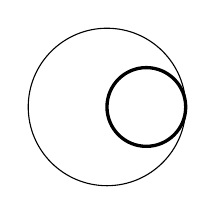
\begin{tikzpicture}[scale=.5]
\draw[very thick] (1,0) circle [radius=1];
\draw[scale=2] (0,0) circle [radius=1]; 
\end{tikzpicture}
\end{tikzshowenvi}
第二行的缩放 \texttt{scale} 是正常图像的 \(0.5\times 2=1\) 倍。

使用负值来实现“翻转”效果,以及使用 \tikzkw{scale around} 来指定缩放中心:
\begin{tikzshow}[very thick]
\draw[thin] (0,0) circle [radius=1];
\draw[xscale=-1] (0,0) rectangle (1,1);
\draw[red, xscale=-1] (0,0) rectangle (1,1);
\draw[blue, scale around={1.5:(1,1)}] (0,0) rectangle (1,1);
\end{tikzshow}

注意,缩放命令 \tikzkw{scale} 并不更改对象的属性,比如点的字体大小、线宽等等。如果想要改变这些,参考\secref{subsec:nodescaling}部分。

\subsubsection{倾斜(slant)*}
倾斜不是一个常用的图像变换。\tikzz\ 中的倾斜指令是 \tikzkw{xslant} 与 \tikzkw{yslant}。简单地解释,\texttt{xslant=k} 会把图像中坐标为 \((x,y)\) 的点变换为 \((x+k\times y, y)\)。
\begin{tikzshow}[very thick,scale=.6]
\draw[help lines] (0,0) grid (4,2);
\draw (0,0) -- (1,1) -- (1,2) -- cycle;
\draw[red, xslant=1.5] (0,0) -- (1,1) -- (1,2) -- cycle;
\draw[blue, xslant=-1] (0,0) -- (1,1) -- (1,2) -- cycle;
\end{tikzshow}

\subsection{裁剪(clip)}
在 \latexline{clip} 命令\RED{之后}的所有绘图都会只显示该裁剪视窗中的部分:
\begin{tikzshow}
\clip (0,0) rectangle (1.1, 1.1);
\draw[red, thick] (0,0) circle [radius=1];
\end{tikzshow}

添加 \tikzkw{draw} 选项可以把 \latexline{clip} 命令的“轮廓”绘制出来\footnote{也可使用 \latexline{draw} 命令并将 \tikzkw{clip} 作为参数,还可将两者作为 \latexline{path} 命令的参数。}:
\begin{tikzshow}
\clip[preaction={draw=red,ultra thick}] (1.2,0) arc [start angle=0, end angle=225, radius=1.2];
\draw (-1,-1) rectangle (1,1);
\draw (-1,1) -- (1,-1);
\end{tikzshow}
上例使用一个非闭合的路径(圆弧)来裁剪,\tikzz\ 会自动将其首尾连接。其中,\tikzkw{preaction} 选项表示在 \latexline{clip} 命令\RED{之前}先沿该路径按传递给其的参数绘制,之后再创建裁剪视窗;这样可以实现视窗轮廓的自定义绘制(因为裁剪只影响其后的绘制命令)。

\subsection{分组(scope)}
\label{subsec:scope}
分组操作允许你对当前组使用参数——这些参数会叠加到全局参数上,并且不影响到组外的对象:
\begin{tikzshowenvi}
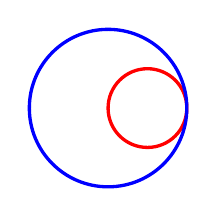
\begin{tikzpicture}[red, very thick, scale=.5]
\draw (1,0) circle [radius=1];
\begin{scope}[blue, scale=2]
\draw (0,0) circle [radius=1];
\end{scope}
\end{tikzpicture}
\end{tikzshowenvi}

\subsection{画布大小}
命令 \latexline{useasboundingbox} 可以

\section{点(node)与文本}

\subsection{点的坐标指定}
使用 \latexline{coordinate} 命令给点命名,便于之后引用。
\begin{tikzshow}
\coordinate (A) at (1,0);
\coordinate (B) at (1,1);
\draw (0,0) -- (A) circle[radius=.5] -- (B) -- cycle;
\end{tikzshow}
\tikzkw{coordinate} 也可以在绘制命令中作为选项使用。

\subsection{点的基本命令}
如需显式地绘制点(即占有面积的点),使用 \latexline{node} 命令,或者 \latexline{path} 命令的 \tikzkw{node} 选项,并配合 \tikzkw{draw} 选项。选项 \tikzkw{shape} 用于指定点的绘制方式。
\begin{tikzshow}
\node at (0,0) [shape=circle, draw] (C) {$p_C$};
\node at (1,0) [rectangle, draw, fill=red] {};
\path[yshift=1cm] (0,.5) node[draw] (A) {$p_A$}
     (1,.5) node[draw] (B) {$p_B$};
\draw (A) -- (B) -- (C);
\end{tikzshow}
选项 \tikzkw{shape} 还可赋值为 \texttt{coordinate},这样在点之间连线时会从点中心开始绘制;但我建议此时直接使用 \tikzkw{coordinate} 命令。

\subsubsection{点的锚点(anchor)}
使用 \tikzkw{anchor} 选项定义锚点位置,可传入的值是 4 个基本方位(east, west, south, north)、4 个复合方位(south west 等),以及 center。或者你可以依次用 left, right, above, below 来替代四个基本方位:
\begin{tikzshow}
\draw[help lines] (0,0) grid (2,2);
\draw (0,0) node [anchor=south west] {$\beta$};
\node at (0,1) [above right] {Here};
\node at (1,0) [above=2pt] {Hi};
\draw (1,2) node [below right=1pt and 8pt] {$1,0$};
\end{tikzshow}
其中,如果像最后一行给出双距离参数,需加载 \pkg{positioning} 库。

也可以直接用数字指定 \tikzkw{anchor} 的角度,\tikzz\ 会自动定位到点边界上对应角度的位置:
\begin{tikzshow}
\draw (0,0) circle [radius=1];
\foreach \x in {1,...,12} {
  \node at (90-30*\x:1) [anchor=270-30*\x] {\x};
}
\end{tikzshow}

点的命名类似 \latexline{coordinate} 的用法:
\begin{tikzshow}
\path node (a) at (0,0) {}
      node (b) at (1,0) {};
\draw (a) -- (b);
\end{tikzshow}

\subsubsection{点的尺寸}
点的大小用 \tikzkw{inner sep} 指定文字到点边框的距离,用 \tikzkw{minimum size} 指定边框的最小尺寸。也可以配合 \tikzkw{text width} 选项指定文本的每行宽度。
\begin{tikzshow}
\tikzset{every node/.style={draw, circle}}
\node (a) {a};
\node[yshift=1cm] (b) {b};
\node[shift={(1,2)}, inner sep=2pt] (c) {c};
\node[xshift=1cm, minimum size=8pt] (d) {d};
\node[shift={(1,1)}, minimum size=8pt, inner sep=0pt] (e) {e};
\end{tikzshow}
注意点 \(d\) 和点 \(e\) 的区别。

\subsection{点的相对放置}
点的相对放置有两种方式。其一如下例,双距离语句需要 \pkg{positioning} 库。
\begin{tikzshow}
\tikzset{every node/.style={draw, circle}}
\draw[help lines] (0,0) grid (3,3);
\node (a) {a};
\node (b) [above=of a] {b};
\node (c) [above right=.5cm and 2cm of b] {c};
\node (d) [below=.5cm of c, on grid] {d};
\draw[red] (b) rectangle (d);
\end{tikzshow}
\tikzkw{on grid} 选项表示从边框而不是点中心开始计算距离,因此 \(b\) 与 \(d\) 的纵坐标不同。另一种方式是使用方位词结合点的名称,组成 \texttt{点名\mbox{.}方位词} 的语法:
\begin{tikzshow}
\node (a) {a};
\node[above] (aa) at (a.north) {a.north};
\end{tikzshow}
上例中的 \tikzkw{above} 选项不是必须的,但往往添加以避免点间的覆盖。

\subsection{点的旁置文本(label/pin)}
旁置文本(或标签)可用上一节的语法画另一个点来实现,但 \tikzkw{label} 或 \tikzkw{pin} 选项更简洁,会直接在主点旁画一个旁置点。对同一个主点画多个 \tikzkw{label} 或 \tikzkw{pin} 都是允许的;它们的区别在于后者会在主点和旁置点之间连一条线。

标签位置的语法是 \texttt{角度\mbox{:}文本}——它还有一个特殊的角度参数 \texttt{center},会将标签放在主点的中心处。你也可以通过 \tikzkw{label distance} 或 \tikzkw{pin distance} 选项来指定距离。
\begin{tikzshow}[every node/.style={draw, circle}]
\draw node[pin={[pin distance=.2cm, pin edge={<-, thick}]above right:$a_{p}$}] (a) at (0,0) {a} 
node[label={[red]30:$b'$}] (b) at (0,1) {b} 
node[label=120:$c'$, label=below:$c''$] (c) at (1.5,1) {c};
\end{tikzshow}
上例中甚至给 \tikzkw{label} 传入了颜色参数。还可以使用 \texttt{every pin, every pin edge} 或 \texttt{every label} 样式设定默认值。

当点被旋转时,参数 \tikzkw{absolute} 可以帮助你定位。如果它的值是 \texttt{true} 或缺省,那么方向不会跟随点而旋转,而是始终以纸面做参照:
\begin{tikzshow}
\tikzset{
    every node/.style={draw, rectangle},
    every label/.style={draw=red, font=\footnotesize}
}
\node[rotate=-80,label=right:label] (a) at (0,0) {normal};
\draw[blue, thick] (0,0) -- (-80:1);
\node[rotate=-80,label={[absolute]right:label}] (b) at (1,0) {absolute};
\draw[blue, thick] (1,0) -- +(0:1);
\end{tikzshow}
左侧标签的锚点(位于红色矩形的左侧边上)在点“normal”右侧边框的中点,而右侧标签的锚点则位于穿过点“absolute”中心的水平向右的线上。\RED{上例中出现了方括号嵌套时,不要忘记添加花括号}。

\subsection{点的沿路径文本}
\subsubsection{显示指定}
将 \tikzkw{node} 选项放于对应的点坐标之后,称为显示(explicitly)指定。

对于沿路径的文本标记,\tikzz\ 预定义了 7 种位置,分别是 \tikzkw{at start/end}, \tikzkw{(very) near start/end},以及缺省时的 \tikzkw{midway}。
\begin{tikzshow}
\draw (0,0) .. controls (.5,2) .. (1.5,2)
  node[at start] {at start}
  node[midway, sloped, above] {midway}
  node[pos=1, right, text width=3ex] {at end};
\end{tikzshow}
上例中的一些参数:
\begin{para}
\item[sloped] 设置文字基线与图中此处的切线平行。
\item[pos] 定量化的位置参数\footnote{并不是严格的空间分点;而是基于首、尾、控制点间向量计算出速度,取其时间分点。很难精确指定。}。比如预定义的 \tikzkw{very near start} 即为 \(0.125\),\tikzkw{near start} 即为 \(0.25\)。
\end{para}

对于交点指定(\tikzkw{|-} 或 \tikzkw{-|}),中点(\tikzkw{midway})即为垂足:
\begin{tikzshow}
\draw (0,0) |- (2,1) \foreach \p in {0,0.5,1} {
  node[pos=\p] {\p}
};
\end{tikzshow}

不同位置放置文本的场合,使用 \tikzkw{auto} 选项,并可以设定 \texttt{left} 或者 \texttt{right} 参数;选项 \tikzkw{swap} 则允许你将其文本放在对称位置。注意:这两个选项\RED{只对沿路径的放置有效}。
\begin{tikzshow}[scale=.5, every node/.style={circle, inner sep=2pt}]
\foreach \x in {1,...,4} {
  \draw (90-90*\x:2) -- (-90*\x:2)
  node[midway, fill=red!30, auto=left] {\x}
  node[midway, fill=blue!30, auto, swap] {\x};
}
\end{tikzshow}

\subsubsection{隐式指定}
路径里点的位置可以隐式(implicitly)指定,放在 \texttt{--} 命令与要连接的点之间即可。只有隐式指定的点才会继承全局参数(因此隐式指定往往可以省略一些参数,比如 \tikzkw{midway})。例子\cite{tikzmanual}:
\begin{tikzshowenvi}
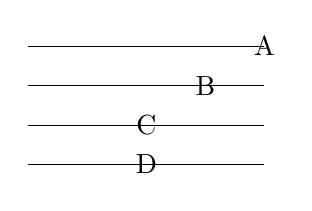
\begin{tikzpicture}[near end]
\draw (0,2.5) -- (3,2.5) node{A};
\draw (0,2) -- node{B} (3,2);
\draw (0,1.5) -- node[midway] {C} (3,1.5);
\draw (0,1) -- (3,1) node[midway] {D} ;
\end{tikzpicture}
\end{tikzshowenvi}
将上述代码中的 \tikzkw{--} 换成 \tikzkw{to} 也可以;通常后者是个更强的命令,在下一节中也会介绍。

\subsection{点之间的连线}
\label{subsec:connectingnodes}
\subsubsection{基础连线}
点之间连线会自动检测点的绘制边界,主要要三种操作方式:
\begin{enumerate}
\item 在点名称后增加小数点和方位词来指定,比如点 a 的左侧就用 \texttt{(a.west)};
\item 使用 \texttt{to} 代替 \texttt{--},并附加 \tikzkw{out} 与 \tikzkw{in} 选项。(如果不附加则会画直线)
\item 使用 \texttt{to} 附加 \tikzkw{bend left/right} 选项。下例中最后一行以 a 到 b 直线方向为角度 0,\texttt{bend left=45} 表示逆时针旋转 $45$ 度作为 \tikzkw{out} 值,旋转 $180-45=135$ 度作为 \tikzkw{in} 值。
\end{enumerate}
\begin{tikzshow}
\tikzset{every node/.style={draw,circle}}
\node (a) {a};
\node (b) [below=of a] {b};
\node (c) [left=of b] {c};
\draw[blue, ->] (c.north) .. controls +(up:1) and +(left:1) .. (a.west); 
\draw[red, ->] (c) [out=315, in=225] to (b);
\draw[->] (a) to [bend left=45] (b);
\end{tikzshow}

\subsubsection{绘制到命令(to)}
除了上面提到的 \tikzkw{to} 命令的用法,它还有以下灵活的使用方式:

使用 \tikzkw{edge node} 来给点之间的连接线添加文本。但更好用的是 \tikzkw{edge label} 命令,表示以 \tikzkw{auto} 选项来自动放置文本;如果换成 \tikzkw{edge label'},则表示以 \tikzkw{auto, swap} 选项放置。
\begin{tikzshow}
\coordinate (a);
\coordinate (b) at ($ (a)+(2,1) $);
\draw (a) to[edge node={node [sloped,above] {ab}}] (b);
\draw (a) to[color=red, bend right=45, edge label=auto, edge label'=swap] (b);
\end{tikzshow}

最后,该命令允许用户以 \tikzkw{to path} 选项来指定绘制方式,并用 \latexline{tikztostart} 表示当前 \tikzkw{to} 命令的起始点,\latexline{tikztotarget} 表示终止点,\latexline{tikztonodes} 表示绘制路径时伴随的点(可省略)。实质上是添加了一个路径分组(花括号内的选项不会应用到外部):
\begin{latex}
{[every to, <options>] <path>}
\end{latex}

例子:
\begin{tikzshow}
\tikzset{selfloop/.style={to path={.. controls +(75:1) and +(105:1) .. (\tikztotarget) \tikztonodes}}}
\node (a) {$a$};
\node[right=of a] (b) {$b$};
\node[below=of b] (c) {$c$};
\draw[->] (a) edge (b) (b) edge[selfloop] node[above] {Hi} (b)  edge (c);
\end{tikzshow}
你可能注意到,上例中虽然定义了 \tikzkw{to path},但使用了 \tikzkw{edge} 而不是 \tikzkw{to};实质上两者的语法有相近之处,但使用 \tikzkw{to} 会导致只有最后一条子路径有箭头。

库 \pkg{topaths} 定义了一些实用的样式,比如在上例中就可以直接使用它预定义 \tikzkw{loop above}。

\subsubsection{边命令(edge)}
边命令的底层形式是,其中 \verb|<path>| 与 \tikzkw{to} 格式相同:
\begin{latex}
\path[every edge, <options>] (\tikztostart) <path>
\end{latex}

因此它将绘制包含同一个点(即 \texttt{\char`\\tikztostart})的所有边。当你想要给每个点的边进行定制时,这会十分有用:
\begin{tikzshow}
\tikzset{every node/.style={draw,circle}}
\node (a) {a};
\node (b) [below=of a] {b};
\node (c) [left=of b] {c};
\draw[thick] (c) edge[red, -latex] (b)
    edge[bend left=45] (a)
    edge[blue, <-] (a);
\end{tikzshow}
提醒一下那些熟悉图论的读者:别忘了尽管最后一行中边的箭头方向是从 a 到 c 的,但仍可以像上面一样用 c 点的 \tikzkw{edge} 命令来绘制。

你还可以连写边命令,并沿边加上文字:
\begin{tikzshow}
\node foreach \name/\angle in {a/0,b/90,c/180,d/270}
    (\name) at (\angle:1.5) {$\name$};
\path[->] (b) edge node[above right] {$5$} (a)
  edge (c)
(c) edge [-,dashed, blue] node[auto] {auto}
  node[auto, swap] {swap} (a)
  edge (d)
(d) edge [red] node[above,sloped] {very}
  node[below,sloped] {red} (a);
\end{tikzshow}
这里用到了之前提及的 \tikzkw{auto} 命令。注意,只要 \tikzkw{path} 命令指定了箭头选项,\tikzkw{edge} 命令绘制的每条边都有箭头。

\subsection{点与画布的缩放}
\label{subsec:nodescaling}


\subsection{作为图像的点(pic)*}
一段绘图代码可能需要复用;如果它比较复杂,可以使用 \latexline{pic} 来重复调用。
\begin{tikzshow}[scale=0.8]
\tikzset{dcircle/.pic={\draw (0,0) circle [x radius=.5, y radius=.8] circle [radius=1];}}
% 两种调用方式
\draw[help lines] (0,-1) grid (2,2);
\pic at (0,0) {dcircle}; 
\path (2,0) pic {dcircle};
\end{tikzshow}
语法非常类似 \tikzkw{node}。其中 \tikzkw{at} 也可以写成 \texttt{[at=\{(0,0)\}]} 这种形式。

\tikzkw{pic actions} 选项用于传入 \texttt{draw, fill, shade, 或 clip} 参数:
\begin{tikzshow}[scale=0.6, transform shape]
\tikzset{circlerect/.pic = {
    \path[pic actions] (.5,.5) circle [radius=.3];
    \draw (0,0) rectangle (1,1);
}}
\draw[red] (0,0) grid (4,2);
\pic [blue, thick] at (.5,.5) {circlerect};
\pic [draw=blue, fill=white] at (2.5,.5) {circlerect};
\end{tikzshow} 
当不传入 \tikzkw{draw} 选项时,圆的 \latexline{path} 命令是不会绘制的;同时注意,因为绘制矩形的是 \latexline{draw} 命令,因此不受\tikzkw{fill} 选项影响。

插入的 \tikzkw{pic} 中的点可以在外部调用,一个例子:
\begin{tikzshow}
\tikzset{mypic/.pic={
  \draw[blue] (0,0) coordinate (-A)
  -- (1,1) coordinate (-B);
}}

\draw[help lines] (0,0) grid (1,2);
\pic (P) {mypic};
\pic (Q) at (0,1) {mypic};
\draw[red] (P-A) -- (Q-B);
\end{tikzshow}
\tikzkw{pic} 定义时用短横命名是为了可读性。调用时语法类似 \tikzkw{node}。

\pkg{quotes} 库支持以加引号字串的方式传入参数,作为 \tikzkw{pic text} 选项的值。比如 \texttt{angles} 这个预定义的 \tikzkw{pic}(由 \pkg{angle} 库支持):
\begin{tikzshow}
\draw (0,-1) coordinate (P1)
  -- (0,0) coordinate (O)
  -- (1,1) coordinate(P2)
  pic [draw, "$\alpha$"] {angle=P1--O--P2};
\end{tikzshow}

一些其他注意:
\begin{feai}
\item 如果有 \texttt{foreach} 语句,\textbf{请放在 \texttt{pic} 定义的首行} 。
\item \tikzkw{pic} 虽说从用法上近似 \tikzkw{node},实质上它是以类似 \tikzz\ \envi{scope} 环境的方式工作的。因此,如果想要其外部的图像变换对其生效,须添加 \tikzkw{transform shape} 选项于 \envi{tikzpicture} 环境。
\item \tikzkw{pic} 对象也能像 \tikzkw{node} 一样,沿路径放置,设置 \tikzkw{at start} 等选项。
\item 将 \tikzkw{pic} 作为选项使用时,添加 \tikzkw{behind path} 或者 \tikzkw{in front of path} 来指定将 \tikzkw{pic} 插入到所在路径的下方或是上方图层。
\item 如果你只是临时使用而不想额外定义,这里有一个使用 \tikzkw{code} 选项的例子\cite{tikzmanual}:
\begin{tikzshow}
\draw (0,0) .. controls(1,0) and (2,1) .. (3,1)
foreach \t in {0, 0.1, ..., 1} {
  pic [pos=\t] {
    code={\draw circle [radius=2pt];}
  }
};
\end{tikzshow}
注意,本例只有一句语句。句中 \tikzkw{pic} 是 \latexline{draw} 命令的选项。
\end{feai}

\section{路径(path)}
虽然我们不常直接使用 \latexline{path} 命令,而是使用它的变体 \latexline{draw} 等,但是我们仍然需要介绍一些它的特性。

最常用的情景就是只声明点,但却不显示地绘制它们:
\begin{tikzshow}
\path coordinate (a)
     coordinate[right=of a] (b)
     coordinate[above=of b] (c);
\draw (a) -- (b) -- (c) -- cycle;
\end{tikzshow}

特别指明,点命令(\tikzkw{node} 或者 \tikzkw{coordinate})总是在路径绘制结束后再绘制的;它们不是路径的一部分。

以下路径命令已在上文(或将在其他小节)进行介绍:
\begin{description}
\item[移动(move-to)指令] 隐式。如 \verb|draw (a) -- (b) (c) -- (d)|,在 b 与 c 间即为移动指令。
\item[直线(line-to)指令] 包括直线指令 \tikzkw{--} 与水平竖直线指令 \tikzkw{|-} 和 \tikzkw{-|}。
\item[曲线(curve-to)指令] 即绘制 \bz\ 曲线的 \tikzkw{.. controls ..} 指令。
\item[绘制到(to)指令] 上文介绍过 \tikzkw{to} 配合 \tikzkw{out, in, bent left} 等命令的用法,参考前文\secref{subsec:connectingnodes}。它实际将指令解释为以上三种指令之一。
\item[几何形状指令] 包括圆或椭圆 \tikzkw{circle}、矩形 \tikzkw{rectangle} 与弧 \tikzkw{arc} 指令。
\item[函数指令*] 包括抛物线 \tikzkw{parabola}、正弦 \tikzkw{sin} 与余弦 \tikzkw{cos} 指令。更复杂的函数会在
\item[网格指令] 即 \tikzkw{grid} 指令。
\item[圆角指令*] 即 \tikzkw{rounded corners} 与 \tikzkw{sharp corners} 指令。
\item[循环指令] 即 \tikzkw{foreach} 指令,具体可参考\secref{subsec:foreach}部分。
\item[暂存指令] 即 \tikzkw{let} 指令,将数据暂存以供语句之后调用。参考\secref{subsec:nodesdistance}部分。
\item[图指令*] 即 \tikzkw{graph} 指令,绘制图、树、网络的命令。参考\secref{sec:network}部分。
\item[图像指令*] 即 \tikzkw{pic} 命令,
\end{description}

本节会介绍除上述指令外的其他路径指令。

\subsection{路径分组}
类似与 \envi{scope} 环境,\tikzz\ 允许在路径中创建一个“分组”,分组中的选项不会影响到分组外部的内容。只需要将想要建立分组的部分用花括号包围即可:
\begin{tikzshow}
\path coordinate (a)
     coordinate[right=of a] (b)
     coordinate[above=of b] (c)
     coordinate[left=of c] (d);
\draw (a) -- (b) {[rounded corners] -- (c) -- (d) {[sharp corners] -- cycle}};
\end{tikzshow}
注意,并不是所有参数都支持分组。例如,每条路径只能有一个颜色,因此在分组中指定另一种颜色是无效的。

\subsection{SVG 指令*}
加载 \pkg{svg.path} 库后,路径中的 \tikzkw{SVG} 选项允许你使用类似网页 \texttt{HTML} 中 \texttt{SVG} 的语法进行绘制。这里不再详细对 SVG 语法做说明,仅给出一个例子:
\begin{tikzshow}
\draw[fill=red!50] svg {M 0 0 L 10 10 h 20 v -10} -- cycle;
\end{tikzshow}
该库只支持真正的 \texttt{SVG} 指令集的主要部分,并不是完全涵盖。

\subsection{绘图指令(plot)}
该指令用于绘制点较多的图,也可以从外部文件读取。

\subsection{计算指令(pgfextra)}
该指令只能用于路径命令内部,运行到此处时路径绘制会挂起,直到运行完该命令内部的部分再继续绘制。一个例子:
\begin{tikzshow}
\newdimen\myloc
\myloc=0cm
\draw (0,\myloc) \pgfextra{\myloc=.5cm}
    circle [radius=\myloc] -- (0,1);
\end{tikzshow}

\section{数学绘制:几何与函数图像}
严格的几何学绘图需要一些特别的命令,比如计算两点间的距离。而且,通常会使用 \tikzkw{coordinate} 而不是 \tikzkw{node} 命令;因为前者并不占用面积,这样画线时才能保证抵达点所在的中心坐标。

\subsection{坐标计算}
库 \pkg{calc} 允许用户使用 \texttt{\$ ... \$} 的形式来计算,并放在一对圆括号中作为坐标:
\begin{tikzshow}
\coordinate[label=below:A] (A);
\coordinate[above right=.5 and 1.5 of A, label=right:B] (B);
\draw (A) -- (B);
\draw ($ (A) + (.3,.4) $) circle (.5);
\end{tikzshow}

\subsection{两点距离计算}
\label{subsec:nodesdistance}
上一节中的半径值是人工计算的。下例让 \tikzz\ 计算距离,并用 \tikzkw{let} 选项将其储存起来,在 \tikzkw{in} 选项的后方进行调用:
\begin{tikzshow}[scale=0.6, transform shape]
\coordinate[label=left:A] (A);
\coordinate[above right=.5 and 1.5 of A, label=right:B] (B);
\draw (A) -- (B);
\draw let \p1 = ($ (B) - (A) $),
         \n{rad} = {veclen(\x1,\y1)}
      in (B) circle[radius=\n{rad}]
         (A) circle[radius=\n{rad}];
\end{tikzshow}
命令 \verb|\p<数字>| 用于存储向量计算结果,比如 \verb|\p1|。对应的,使用 \verb|\x1| 或者 \verb|\y1| 可以调用向量的两个坐标值。而 \verb|\n<数字>| 则用于存储数值。此外,命令 \tikzkw{veclen} 用于计算向量的欧式长度 \(\sqrt{x^2+y^2}\)。  

如果不想使用数字命名,可以像上例的存储数值一样使用字符串;不过这样命名需要加上花括号。事实上,已知圆心 $A$ 和圆周上一点 $B$,有更简单的画圆方法,参考\secref{subsec:circlethrough}部分的内容。

\subsection{$\lambda$分点与垂线}
\subsubsection{比例分点}
分点是几何中常用的概念,\pkg{calc} 库支持像 \pkg{xcolor} 混合颜色类似的命令:\verb|<点A>!<分点比例>![角度]<点B>|,不同的是“角度”会将分点位置绕 A 旋转一个角度。将它还可以用最后一行中链式的方法进行连写:
\begin{tikzshow}
\coordinate[label=left:A] (A);
\coordinate[above right=.5 and 1.5 of A, label=right:B] (B);
\coordinate (X) at ($ (A)!0.5!(B) $);
\coordinate[label=above:C] (C) at ($ (X)!{sqrt(3)}!90:(B) $);
\path[draw=black, fill=blue!20] (A) -- (B) -- (C) -- cycle;
\node[draw=black, fill=red!20, circle through=(X)] at ($ (A)!0.5!(B)!{tan(30)}!90:(B) $) {};
\end{tikzshow}

\subsubsection{距离分点}
你也可以用(直线段)分点距离代替分点比例,加上单位即可:
\begin{tikzshow}
\coordinate[label=left:A] (A);
\coordinate[above right=.5 and 1.5 of A, label=right:B] (B);
\coordinate (C) at ($ (A)!0.5!(B) $);
\draw ($ (C)!1cm!90:(B) $) edge (B) edge (A)
     edge[dashed] node[above, sloped, font=\footnotesize] {1cm} (C);
\end{tikzshow}

\subsubsection{投影分点(垂线)}
用投影点代替分点比例,则得到该点向连线段的投影:
\begin{tikzshow}
\coordinate[label=left:A] (A);
\coordinate[above right=.5 and 2 of A, label=right:B] (B);
\coordinate[above right=1 and .5 of A, label=above:C] (C);
\draw (A) -- (B) -- (C) -- cycle;
\draw[red] (C) -- ($ (A)!(C)!(B) $);
\end{tikzshow}

\subsection{过某点的圆*}
\label{subsec:circlethrough}
使用 \pkg{through} 库可以方便地画出给定圆心和过某点的圆,而不需要做两点距离计算:
\begin{tikzshow}[scale=0.6]
\coordinate[label=below left:A] (A);
\coordinate[above=1 of A, label=above right:B] (B);
\draw (A) -- (B);
\node[draw, circle through=(B), label=left:C] at (A) {};
\node[draw, circle through=(A), label=right:D] at (B) {};
\end{tikzshow}
注意,\tikzkw{circle through} 仅仅适用于 \tikzkw{node} 命令。

\subsection{交点}
在\secref{subsec:intersection}中已经介绍过交点的使用,包括 \tikzkw{-|} 指令与 \pkg{intersections} 库的一些用法。这里的例子更复杂一些,也复习了之前等分点的用法:
\begin{tikzshow}
\tikzset{small/.style={draw, circle, fill=black, inner sep=1pt}}
\coordinate[label=left:A] (A);
\coordinate[above right=.5 and 1.5 of A, label=right:B] (B);
\coordinate[label=below:C] (C) at ($ (A)!0.5!(B) $);
\coordinate (D) at ($ (C)!2!90:(B) $);
\coordinate (E) at ($ (C)!2!-90:(B) $);
\draw (A) -- (B);
\draw[red, name path=Lv] (E) -- (D);
\node[draw, circle through=(B), name path=Ca] at (A) {};
\path[name intersections={of=Lv and Ca, by={[label=above right:D]D, [label=right:E]E}}];
\foreach \x in {A,C,D,E}
  \node[small] at (\x) {};
\end{tikzshow}
注意上例中的 \latexline{path} 命令虽声明了交点,但没有画任何内容。

\section{图与网络绘制*}
\label{sec:network}

\section{属性}
\label{sec:tikz-property}

\subsection{线宽}
\tikzz\ 预定义了 7 种线宽,从细到粗是:\tikzkw{ultra thin}, \tikzkw{very thin}, \tikzkw{thin}, \tikzkw{semithick}, \tikzkw{thick}, \tikzkw{very thick}, \tikzkw{ultra thick}。或者利用 \tikzkw{line width} 选项指定。
\begin{tikzshow}
\draw[ultra thin] (0,0) -- (1,0);
\draw[ultra thick] (1,0) -- (2,0);
\draw[line width=10pt] (0,1) -- (2,1);
\end{tikzshow}
初始线宽是 0.4pt;两个 \tikzkw{ultra} 线宽分别是 0.1pt 与 1.6pt。

\subsection{线型}
\tikzz\ 预定义了 4 种基本线型:\tikzkw{dashed}, \tikzkw{dotted}, \tikzkw{dash dot}, \tikzkw{dash dot dot}。它们还可以配合 \tikzkw{loosely} 或者 \tikzkw{densely} 进行微调。
\begin{tikzshow}
\draw[dashed] (0,0) -- (1,0);
\draw[dotted] (0,-0.5) -- (1,-0.5);
\draw[dash dot] (0,-1) -- (1,-1);
\draw[dash dot dot] (0,-1.5) -- (1,-1.5);
\draw[loosely dashed] (0,-2) -- (1,-2);
\draw[densely dotted] (0,-2.5) -- (1,-2.5);
\end{tikzshow}

如果的确需要深度自定义,请使用 \tikzkw{dash pattern} 自定义线型,并可配合 \tikzkw{dash phase} 指定线型的起始位置。
\begin{tikzshow}
\draw[dash pattern=on .1cm off .25cm on .25cm off .15cm, dash phase=1cm] (0,0) -- (3,0);
\end{tikzshow}

有时你可能会看到一些复杂的装饰线(需要 \pkg{decorations} 库),比如:\tikz{\draw [->,decorate,decoration=snake] (0,0) -- (2,0)}。请参考\secref{subsec:deco}。

\subsection{线尾(line cap)*}
如果线宽度较大,不同的线尾 \tikzkw{line cap} 明显对应不同的效果:
\begin{tikzshow}[every label/.style={font=\footnotesize}]
\foreach \offset/\s in {0/rect, .5cm/butt, 1cm/round} {
    \draw[yshift=\offset,line width=5pt, line cap=\s] (0,0) -- (1,0)  node[label=right:\s] {};
    \draw[yshift=\offset, white] (0,0) -- (1,0);
}
\end{tikzshow}

\subsection{线交(line joint)*}
连续画线时(非连续画线处此选项无效),可以设置 \tikzkw{line joint}:
\begin{tikzshow}[every label/.style={font=\footnotesize}]
\foreach \offset/\s in {0/round, 1.25cm/bevel, 2.5cm/miter} {
    \draw[xshift=\offset,line width=5pt, line join=\s] (0,0) -- (.5,1) node[label=above:\s] {} -- (1,0)  ;
}
\end{tikzshow}
其中 \tikzkw{miter} 线交在锐角时会产生一个非常“尖”的效果,可以设置 \tikzkw{miter limit} 参数来设置一个角度值,使小于该角度的 \tikzkw{miter} 线交自动转变为 \tikzkw{bevel} 形式。

\subsection{箭头}
\tikzz\ 中的箭头使用的细节多到可以单独开一个章节,但我并不想全部详尽地介绍。用大于或小于号表示箭头的指向,用竖线表示是否加上截断符号。一些基本的样例:
\begin{tikzshow}
\draw[->|] (1,3) -- (2,3);
\draw[stealth-] (1,2) -- (2,2);
\draw[->,>=stealth, line width=3pt] (1,1) arc [start angle=90, end angle=30, radius=1];
\draw[<->] (.5,4) -- (.5,0) -- (2.5,0);
\end{tikzshow}
其中,用 \texttt{>=stealth} 或 \texttt{-stealth} 的方式指定了箭头末端的类型为 \texttt{stealth}。你也可以将它们作为整个 \envi{tikzpicture} 环境的参数进行传递。

\tikzz\ 的 \pkg{arrows.meta} 库包含很多箭头,读者可以自行查阅。

\subsection{绘制颜色}
在绘制网格一节,已经使用过 \texttt{lightgray} 作为网格的绘制颜色;当时省略了 \tikzkw{color} 选项。该选项设定\RED{除了 shading 外的所有}颜色,包括绘制、填充等:
\begin{tikzshow}
\path[draw,fill,red!50] (0,0) -- (1,0) circle[radius=.5];
\end{tikzshow}
注意:单独使用 \latexline{draw} 或者 \latexline{fill} 只会执行绘制或填充其一,除非详细指定局部的参数。

可以使用 \tikzkw{draw} 来单独指定绘制的颜色:
\begin{tikzshow}
\draw[draw=red!50!white, ultra thick] (0,0) rectangle (1,1);
\end{tikzshow}
其中,双感叹号加数字是表示插值比例为 0.5;\pkg{xcolor} 宏包支持该语法。常用的颜色包括:
\begin{tikzshow}
\tikzset{every pin/.style={pin distance=.5cm, font=\footnotesize, inner sep=0pt}}
\draw (0,0) circle[radius=1];
\foreach \c[count=\i] in {red,green,blue,cyan,magenta,yellow,black,
lightgray,gray,darkgray,white,brown,
lime,olive,orange,pink,purple,teal,violet}
\node[circle,draw=black, fill=\c, pin={[pin edge={draw=\c, thick}] 90-360/19*\i:\c}] at (90-360/19*\i:1cm) {};
\end{tikzshow}

在 \tikzz\ 环境内部,还可以使用 \latexline{colorlet} 或者 \latexline{definecolor} 自定义颜色(它们实际上是 \TeX\ 指令),例如:
\begin{latex}
\colorlet{linecolor}{red!60!black}
\definecolor{fillcolor}{rgb}{1,0.5,1}
\end{latex}

\subsection{单色填充}
填充命令 \latexline{fill} 只能使用于闭合区域,\textbf{且不绘制区域边界}。你可以在一般绘制命令的末尾添加 \tikzkw{cycle} 来创建一个闭合对象:
\begin{tikzshow}
\fill[green] (0,0) -- (1,0) -- (1,1) -- cycle;
\end{tikzshow}

在填充的同时绘制\footnote{准确地说,\latexline{filldraw} 命令是先绘制再填充。},使用 \latexline{filldraw} 命令,并分别指定绘制和填充颜色:
\begin{tikzshow}
\filldraw[draw=black, fill=cyan] (0,0) -- (2,0) arc (0:30:2);
\end{tikzshow}
\tikzkw{filldraw} 填充的区域会比用 \tikzkw{fill} 稍大一些,因为前者考虑了线宽。

要了解填充的细节,需要介绍两个区域特性:
\subsubsection{非零区域}
该特性是默认的区域特性。\tikzz\ 使用计数器的方式来区分路径的内部与外部。对于某点的判断,它会从该点发射一条到无穷远的射线;如果沿途的路径是从左到右(顺时针)地与这条射线相交,那么计数器加一;反之减一。最后计数器如果是零,那么该点在路径外部;否则,它在区域内部。

下例逆时针地绘制了小矩形、顺时针地绘制了完全围住小矩形的大矩形。这样小矩形的内部被识别为“外部”,因此未被填充。
\begin{tikzshow}
\filldraw[fill=blue!50] (0,0) -- (0,.5) -- (1,.5) -- (1,0) -- cycle
  (-.5,-.5) -- (1.5,-.5) -- (1.5,1) -- (-.5,1) -- cycle;
\end{tikzshow}

\subsubsection{奇偶区域}
奇偶区域也会发射一条射线,但只要遇到路径就会计数器加一。利用区域的奇偶性填充,使用 \tikzkw{even odd rule}:
\begin{tikzshow}
\fill[even odd rule, blue] (0,0) -- (2,0.5) -- (1,1) circle (0.25);
\end{tikzshow}

\subsection{图案与图像填充*}
在指定了 \tikzkw{pattern} 选项时,它会自动进行填充操作(即使你使用的是 \latexline{draw} 命令)。要使用图案填充,请加载 \pkg{patterns} 库。
\begin{tikzshow}
\draw[pattern=dots, pattern color=red] (0,0) rectangle (1,1);
\end{tikzshow}

图像填充允许你使用外部图像,或者一般的 \tikzz\ 命令。注意配合 \tikzkw{path picture bounding box} 使用。

\begin{tikzshow}
\draw[pattern=dots, pattern color=red] (0,0) rectangle (1,1);
\end{tikzshow}

\subsection{渐变填充*}
使用 \latexline{shade} 命令控制渐变填充,

\subsection{透明度*}
p169

\subsection{双线*}
双线选项在某些场合也是实用的。可以用 \tikzkw{double distance} 指定双线内间距(默认 0.6pt),或者用 \tikzkw{double distance between line centers} 指定双线的中心间距。
\begin{tikzshow}
\draw[double] (0,0) -- (1,1);
\draw[draw=white, double=cyan] (1,0) -- (0,1);
\draw[double distance=1pt] (1.2,0) -- (1.2,.5);
\draw[double distance=1pt,thick] (1.2,.5) -- (1.2,1);
\end{tikzshow}
上例的 \tikzkw{draw} 指定为白色,实质创造一种“从上方穿过”的效果。

还有一个特殊的双线选项 \tikzkw{double equal sign distance},可以将双线间距设置成与当前字体的等号($=$)间距一致。

\section{样式与高级控制}

\subsection{样式(style)}
如果某种属性需要用来反复作图,可以把它自定义为样式:

上文中出现过的 \texttt{help lines},就是 \tikzz\ 预定义的一种样式。其相当于于:
\begin{latex}
\begin{tikzpicture}[help lines/.style={line width=0.2pt,gray}]
...
\end{tikzpicture}
\end{latex}

你也可以在进入 \tikzz\ 环境后(或在文档导言区),使用 \latexline{tikzset} 命令来定义。

\subsection{循环语句(foreach)}
\label{subsec:foreach}
\tikzz\ 支持循环语句,这一点对于科技绘图来说十分重要。
\begin{tikzshow}[place/.style={circle, draw, fill=black, minimum size=5pt, inner sep=0pt}]
\foreach \x in {1,2,3} {
    \node at (\x, 0) [place] {};
    \draw (\x, 0) circle [radius=1/\x];
}
\end{tikzshow}

有时候我们需要循环一个等差数列,这时候使用 \ldots\ 即可。\tikzz\ 会将 \(a,b,\ldots,c\) 识别为从 \(a\) 到 \(c\) 以 \(b-a\) 为公差的等差数列;如果你不指定 \(b\),那么默认以 \(1\) 为公差。
\begin{tikzshow}[place/.style={circle, draw, fill=black, minimum size=5pt, inner sep=0pt}]
\foreach \x in {1,1.5,...,3,4} {
    \node at (\x, 0) [place] {};
    \draw (\x, 0) circle [radius=\x/8];
}
\end{tikzshow}
上例中的 \(4\) 不在数列内,这样写是允许的。数列后也可以接另一个数列。

大部分需要知道“循环到列表第几个”的场合,都可以配合移动画笔或相对坐标命令实现:
\begin{tikzshow}[scale=.5]
\draw[red] (0,0) grid (3,3);
\foreach \x/\y in {0,1/2,2}
  \draw (\x, \y) +(.5,.5) circle [radius=.4];
\end{tikzshow}
上例同时循环了多个变量,中间用斜线分隔;它们分别按照列表中斜线分隔后的对应值进行循环。如果某一位置的列表提供值的个数小于变量的个数,那么“多出”的变量将都取最后一个值。

此外,如果 \latexline{foreach} 内部只有一条语句,像上例一样不加花括号也可以。

\subsection{图层*}
一般情况不会用到此指令。但有时你需要先画完上层的内容才能确定下层元素的尺寸,这时候可能需要图层\cite{tikzmanual}(需要 \pkg{backgrounds} 库):
\begin{tikzshow}
\tikzset{every node/.style={draw,circle,inner sep=.1cm, minimum size=.8cm}}
\foreach \x/\pos in {{a/(0,0)},{b/(1.5,0)},{c/(1,-1)}}
    \node (\x) at \pos {\x};
\draw (b.east) .. controls +(0:1) and +(0:1) .. (c.east);
\begin{scope}[on background layer]
    \node[draw=none,fill=lightgray, rectangle, fit=(b) (c)] {};
\end{scope}
\end{tikzshow}
上例中还使用了 \pkg{fit} 库,用来创建一个“遮盖”点 b 和点 c 的背景点——这个点的矩形边框被 \tikzkw{fit} 命令处理成图中的大小。

\subsection{装饰*(decorations)}
\label{subsec:deco}
最简单的装饰是蛇形线\cite{tikzmanual},需要 \pkg{decorations.pathmorphing} 库:
\begin{tikzshow}
\draw[->,decorate,decoration=snake] (0,0) -- (2,0);
\end{tikzshow}

通常,我们希望在线段结束就终止装饰(否则会蛇形绘制到线段末尾,这可能引起困惑)。下面是一个复杂的例子:
\begin{tikzshow}
\draw[->, decorate, decoration={snake,amplitude=.4mm,segment length=4mm,post length=2mm}] (0,0) -- (3,0)
    node[above, align=center, midway, text width=2.5cm, font=\footnotesize] {
        multiline text controlled by \texttt{text width} option of \textcolor{blue}{node}
    };
\end{tikzshow}
大部分的参数都比较好理解。\tikzkw{amplitude} 控制波动的强弱,\tikzkw{segment length} 控制一个周期的长度,\tikzkw{post length} 控制在终点之前何处结束装饰。

\subsection{随机数*}
\tikzz\ 使用 \tikzkw{rand} 来生成从 $-1$ 到 $1$ 的随机数(服从均匀分布);如果使用 \pkg{calc},你还可以在指定坐标时使用 \texttt{(\$...\$)} 并在其中做坐标计算: 
\begin{tikzshow}
\makeatletter\def\pgfcurrentseed{
  \pgfmathparse{\pgfmath@rnd@z}\pgfmathresult
}\makeatother
\coordinate [label=left:$A$] (A) at (.5*rand,.5*rand);
\draw (0,0) node[below=1] {\pgfcurrentseed} circle [radius=1];
\coordinate [label=left:$B$] (B) at ($ (0,0) + (rand,rand)$);
\path (0,0) node[above=1] {\pgfcurrentseed};
\end{tikzshow}
上例中在 \TeX\ 底层中使用 pgf 命令从 \latexline{pgfmath@rnd@z} 中读取当前随机数种子的值,并赋给自定义命令。每次使用 \tikzkw{rand} 命令都会改变随机数种子的值。

\subsection{外部数据文件*}

\section{实用范例}
\label{sec:tikz-eg}
本节通过例子的方式,向读者展示 \tikzz\ 的常用情形。

% Appendices

% 参考文献
\bibliography{Bib}

% 附录
\clearpage %清空浮动体队列,并开始新一页。
\appendix
% 重定义附录的chapter样式
\renewcommand{\chaformat}[1]{%
	\parbox[b]{.5\textwidth}{\raggedleft\bfseries \S 附录 \\ \vspace{0.2ex} #1} \quad\rule[-12pt]{2pt}{70pt}\quad
	{\fontsize{60}{60}\selectfont\thechapter}}

\chapter{注音符号}
\label{app:phonetic}
% 这里不用>{\ttfamily}而用\verb是为了减少报错可能
\begin{center}
\tabcaption{注音符号与特殊符号}
\begin{tabular}{|*{4}{>{\centering}p{3em} @{-\hspace{1em}} p{3em}|}}
\hline
\texttt{样式} & 命令 & \texttt{样式} & 命令 & \texttt{样式} & 命令 & \texttt{样式} & 命令 \\
\hline
\=o  & \verb|\=o|  & \'o  & \verb|\'o|  & \v o & \verb|\v o|  & \`o   & \verb|\`o|  \\
\^o  & \verb|\^o|  & \"o  & \verb|\"o|  & \.o  & \verb|\.o|   & \H o  & \verb|\H{o}| \\
\d o & \verb|\d{o}| & \u o & \verb|\u{o}| & \b o & \verb|\b{o}|  & \t oo & \verb|\t{oo}|\\
\multicolumn{2}{|c@{\bf --}}{$\tilde{o}$} & \multicolumn{2}{@{\bf --}c|}{\tt{\$$\backslash$tilde\{o\}\$}} &%
\multicolumn{2}{c@{\bf --}}{$\hat{o}$}    & \multicolumn{2}{@{\bf --}c|}{\tt{\$$\backslash$hat\{o\}\$}}\\
\multicolumn{8}{|c|}{} \\
\o  & \verb|\o|  & \O  & \verb|\O|  & \i  & \verb|\i|  & \j  & \verb|\j| \\
\aa & \verb|\aa| & \AA & \verb|\AA| & \ae & \verb|\ae| & \AE & \verb|\AE|\\
\oe & \verb|\oe| & \OE & \verb|\OE| & !`  & \verb|!`|  & ?`  & \verb|?`| \\
\hline
\end{tabular}
\end{center}

\mbox{}

\begin{center}
\tabcaption{国际音标输入表(部分)}
\begin{tabular}{|*{3}{>{\rmfamily}c !{-} >{\ttfamily}p{7.5em}|}}
\hline
\texttt{样式} & 命令 & \texttt{样式} & 命令 & \texttt{样式} & 命令 \\
\hline
\textdzlig & \char92textdzlig & \textesh & \char92textesh & \textteshlig & \char92textteshlig \\
\textdyoghlig & \char92textdyoghlig & \textturnv & \char92textturnv & \textschwa & \char92textschwa \\
\textscriptg & \char92textscriptg & \texttheta & \char92texttheta & \textupsilon & \char92textupsilon \\
\textscripta & \char92textscripta & \dh & \char92dh & \textepsilon & \char92textepsilon \\
\textopeno & \char92textopeno & \textyogh & \char92textyogh & \ng & \char92ng \\
\hline
\multicolumn{2}{|c|}{重音} & \multicolumn{2}{c|}{次重音} & \multicolumn{2}{c|}{长音节} \\
\textprimstress & \char92{}textprimstress & \textsecstress & \char92textsecstress & \textlengthmark & \char92textlengthmark \\
\hline
\end{tabular}
\end{center}

\textit{注:\texttt{\char92dh}命令在非CJK文档中有时编译会出现问题}.

\chapter{建议与其他}

除了参考文献列表中给出的书籍以外,我还推荐你用控制台在\TeX{} Live中能找到的以下书籍:

\medskip\begin{para}
\item[texdoc usrguide] \TeX\ Live自带的用户手册.
\item[texdoc clsguide] \TeX\ Live自带的文档类和宏包编写手册.
\item[texdoc fntguide] \TeX\ Live自带的字体使用手册.
\item[texdoc symbols-a4] 一份速查表,基本上所有的\LaTeX\ 字符命令都在这里了.
\item[texdoc latexcheat] 很有趣的命令表,只有两页.
\item[texdoc impatient] \emph{\TeX{} for the Impatient}, 一本介绍底层\TeX\ 的书.这也是我阅读的第一本\TeX\ 书,Knuth的\emph{The \TeX\ book}虽然血统正但是难啃啊.本书中译本在:\url{https://bitbucket.org/zohooo/impatient/wiki/Home}
\item[texdoc texbytopic] \emph{\TeX{} by Topic}, 个人觉得不如上面那本,但也许只是叙述方式不一样吧.
\end{para}
\bigskip

\noindent 你可能还需要的功能:
\begin{description}
\item[\pkg{mhchem}] 该宏包用于输入化学式,提供了\latexline{ce}命令.
\end{description}

% \tikzz\ 索引
%\setlength{\columnseprule}{0pt}
%\printindex

\end{document}
